\documentclass[11pt,letterpaper]{article}

% ===== Packages =====
\usepackage[margin=1in]{geometry}
\usepackage{amsmath, amssymb, amsthm}
\usepackage{graphicx}
\usepackage{booktabs}
\usepackage{caption}
\usepackage{subcaption}
\usepackage{xcolor}
\usepackage{hyperref}
\usepackage[round,authoryear]{natbib}
\usepackage{microtype}
\usepackage{enumitem}
\usepackage{titlesec}
\usepackage{fancyhdr}
\usepackage{listings}
\usepackage{array}

% ===== Settings =====
\hypersetup{
  colorlinks=true,
  linkcolor=black,
  citecolor=blue!50!black,
  urlcolor=blue!50!black,
}

\setlength{\parindent}{0pt}
\setlength{\parskip}{6pt plus 1pt minus 1pt}
\renewcommand{\baselinestretch}{1.05}

\titleformat{\section}{\large\bfseries}{\thesection}{0.6em}{}
\titleformat{\subsection}{\normalsize\bfseries}{\thesubsection}{0.6em}{}

\pagestyle{fancy}
\fancyhf{}
\rhead{\small StochastiQ}
\lhead{\small MGT 6081-A Final Project}
\rfoot{\small \thepage}

\captionsetup{font=small,labelfont=bf,format=plain}

\lstset{
  basicstyle=\small\ttfamily,
  breaklines=true,
  frame=single,
  framesep=4pt,
  rulecolor=\color{black!30},
  showstringspaces=false,
}

% ===== Document =====
\begin{document}

% ----- Title page -----
\begin{titlepage}
\centering
\vspace*{1cm}
{\Huge\bfseries StochastiQ\par}
\vspace{0.4cm}
{\Large Multi-Model Portfolio Optimization with Stochastic Simulation,\par
Options Overlay, and Regime-Conditional Validation\par}
\vspace{1.5cm}

{\large\bfseries Team Members\par}
\vspace{0.3cm}
{\large
Anay Abhijit Joshi \\[2pt]
Vidhi Chaturvedi \\[2pt]
Sriya Nelluri \\[2pt]
Himanshu Bhatt \\[2pt]
}
\vspace{1cm}

{\large\bfseries Course\par}
\vspace{0.2cm}
{\large MGT 6081-A: Derivative Securities\par}
\vspace{0.3cm}
{\large\bfseries Instructor\par}
\vspace{0.2cm}
{\large Prof.\ Satyajit Karnik\par}
\vspace{0.5cm}
{\large Georgia Institute of Technology\par M.S.\ in Quantitative and Computational Finance\par Spring 2026\par}

\vfill

\begin{center}
\fbox{\parbox{0.88\textwidth}{
\centering\small
\textbf{Project Direction.} This work was carried out under \emph{Project Idea 6} (independent direction, approved in advance by the instructor). Our project incorporates the full blueprint of \emph{Project Idea 1} —stochastic simulation of a portfolio under GBM, Merton, CEV and Heston with weight reoptimization and an options overlay— and substantially extends it with statistically rigorous out-of-sample validation, Hidden-Markov-Model regime conditioning, and coherent-risk-measure (CVaR) decomposition. \\[5pt]
\textbf{Repository.} All source code, notebooks, processed data, and reproducible artifacts are publicly available at \\
\url{https://github.com/anay-a-joshi/StochastiQ} \\[2pt]
under the MIT License.
}}
\end{center}
\vspace{0.5cm}
\end{titlepage}

% ----- Executive Summary -----
\section*{Executive Summary}
\addcontentsline{toc}{section}{Executive Summary}

We built and validated an end-to-end pipeline for multi-model portfolio construction: data ingestion of seven assets over five years, calibration of four stochastic-process models (GBM, Merton jump-diffusion, CEV, Heston stochastic volatility), correlated Monte Carlo simulation with $5{,}000$ paths per model, per-model and three model-robust portfolio optimizations, a Black-Scholes-Merton options overlay covering covered call, protective put, and collar strategies, statistically rigorous out-of-sample validation using stationary block-bootstrap inference, and a regime-conditional analysis using a two-state Gaussian Hidden Markov Model (HMM) with external validation against the CBOE Volatility Index (VIX).

The central empirical question we set out to answer is whether a model-robust portfolio (specifically, our min-max worst-case allocation across the four stochastic-process models) outperforms the naïve $1/N$ benchmark on a realistic out-of-sample window for a seven-asset universe of large-cap U.S.\ equities and broad-market ETFs. We find two distinct results, which we report honestly:

\textbf{Phase 6 (unconditional).} On the 332-day out-of-sample window (2025-01-02 through 2026-04-30), the paired stationary block-bootstrap test on the difference of Sharpe ratios returns $\widehat{\Delta} = -0.443$ with 95\% confidence interval $[-1.40,\, +0.21]$ and $p = 0.288$. This is the textbook \citet{demiguel2009optimal} finding: estimation noise dominates optimization gains over short horizons, and a single window cannot reject the null that robust and naïve allocations have equal risk-adjusted performance.

\textbf{Phase 7 (regime-conditional).} A two-state Gaussian Hidden Markov Model fit on training-period SPY returns cleanly separates a ``Calm'' state (annualized volatility 14.5\%) from a ``Stress'' state (47.0\%), with the Stress state showing a regime-conditional mean VIX of 35.3 versus 19.6 in Calm —a $+15.7$-point premium that anchors the latent labels to the canonical fear-gauge. Within-regime paired bootstrap tests on the Sharpe difference remain underpowered; even after Holm-Bonferroni multiple-testing correction across 14 paired tests, no Sharpe difference rejects the null. However, the regime-conditional CVaR$_{95}$ comparison tells a different story: \emph{seven of seven} optimized portfolios show better Stress-day CVaR than the equal-weighted benchmark, with the Per-Heston portfolio leading at $-5.65\%$ versus the equal-weighted $-6.27\%$ (a 62-basis-point reduction in expected worst-tail loss per Stress day). Crucially, all seven optimized portfolios are \emph{worse} than the benchmark on Calm-day CVaR, an explicit cost-of-insurance pattern consistent with the design intent of any tail-risk-targeted strategy.

\textbf{Headline interpretation.} In our opinion, the strongest finding of this project is methodological: a strategy designed to manage state-contingent risk must be evaluated using a state-contingent risk metric. Sharpe ratio averages over both regimes and is not the right object for evaluating a tail-risk-oriented design. CVaR, anchored in the coherent-risk-measure framework of \citet{artzner1999coherent}, is. This conclusion maps directly to the broader MGT 6081 framework: derivative-overlay strategies have payoffs contingent on market state and require state-conditional evaluation.

\textbf{On Project 1's question of which model is most pertinent for the future.} Based on Stress-regime tail-risk performance, we conclude that the \emph{Heston} stochastic-volatility model is the most pertinent for forward-looking portfolio construction within this asset universe (best Stress CVaR by a meaningful margin), with Merton jump-diffusion a close second (60 bps improvement vs.\ EW). Both capture features of the empirical return distribution (vol clustering, leverage, jumps) that GBM and CEV cannot. We discuss this in detail in Section 9.2.

\textbf{Honest limitations we disclose explicitly.} Our 16-month out-of-sample window contains only 15 HMM-identified Stress days, far below the minimum sample size required for stable bootstrap inference. The Phase 7 statistical tests are therefore conducted in-sample on training data, with the OOS window presented as descriptive only. The Min-max optimizer converged to weights identical to our per-GBM allocation, indicating that GBM was the binding worst-case model in the min-max formulation —a candid disclosure relevant to interpretation. The HMM-vs-realized-volatility classifier agreement is weak ($\kappa = 0.23$) but expected, since the two methods optimize different objectives. We address each of these in Section 9.4.

\newpage
\tableofcontents
\newpage

% =================================================================
% 1. Introduction
% =================================================================
\section{Introduction}

\subsection{Project Direction: Building on Project~1 with the Latitude of Project~6}

This project was carried out under \emph{Project Idea 6} (independent direction, approved in advance by the instructor). It is structured as a substantial extension of \emph{Project Idea 1}, whose blueprint we adopted in full and then expanded along several dimensions that we believe were necessary to draw scientifically meaningful conclusions.

The core of Project Idea 1 was: pick a portfolio of stocks/ETFs, build a minimum-variance/maximum-return baseline, simulate forward under GBM, Merton, CEV and Heston, reoptimize the weights to perform best across the model-conditional distributions, add a suitable options overlay to improve the Sharpe ratio, and finally take a view on which models are most pertinent for the future. Every single one of those components appears in our work:

\begin{itemize}[leftmargin=*,nosep,topsep=4pt]
  \item Markowitz mean-variance baseline with five canonical portfolios (Section~3 / Phase~2).
  \item Calibration of GBM, Merton, CEV and Heston for each of seven assets (Section~4 / Phase~3).
  \item Forward Monte Carlo simulation under each model with cross-asset correlation injection (Section~5 / Phase~4).
  \item Per-model and model-robust portfolio reoptimization (Section~5 / Phase~4).
  \item BSM options overlay across three classical strategies: covered call, protective put, collar (Section~6 / Phase~5).
  \item A direct answer to ``which model is most pertinent for the future,'' grounded in our regime-conditional tail-risk evidence (Section~9.2).
\end{itemize}

What makes this project an instance of Project Idea 6 rather than Project Idea 1 are the additions we made on top:

\begin{itemize}[leftmargin=*,nosep,topsep=4pt]
  \item \textbf{Five years of training data} (1{,}257 trading days, 2020-01-03 to 2024-12-31) rather than one year, so that calibration is anchored across multiple regime episodes (COVID 2020, the 2022 inflation/rate-hike drawdown, the 2023-2024 AI rally).
  \item \textbf{A dedicated 16-month out-of-sample window} (332 trading days, 2025-01-02 to 2026-04-30) reserved for validation and never touched during model fitting or weight selection.
  \item \textbf{A statistically rigorous validation framework} based on the stationary block-bootstrap of \citet{politis1994stationary}, with paired Sharpe-difference tests and pre-registered decision rules.
  \item \textbf{A Hidden Markov Model regime-conditional analysis} \citep{hamilton1989new} that decomposes performance by latent market state and validates the regime labels externally against the VIX.
  \item \textbf{A coherent-risk-measure (CVaR) decomposition} \citep{artzner1999coherent, rockafellar2002conditional} alongside Sharpe ratio, since CVaR is the appropriate metric for evaluating a tail-risk-targeted strategy.
  \item \textbf{Holm-Bonferroni multiple-testing correction} \citep{holm1979simple} on the 14 paired tests we conducted, to protect against false positives from running many comparisons.
\end{itemize}

In our opinion, these additions transform Project~1 from a portfolio-construction exercise into a falsifiable empirical investigation —which is what we believe a master's-level QCF final project should look like. The instructor confirmed in advance that this hybrid scope qualified as Project~6.

\subsection{The Central Empirical Question}

Our headline empirical question is the following: \emph{does a model-robust portfolio constructed by optimizing the worst-case Sharpe ratio across four stochastic-process models outperform the naïve $1/N$ benchmark out-of-sample, for a realistic seven-asset universe?}

We chose this question for two reasons. First, it is a direct test of the Project~1 hypothesis that multi-model robust optimization improves on simpler approaches. Second, it puts our framework on a collision course with the well-known DeMiguel-Garlappi-Uppal puzzle —the empirical regularity that elaborate optimization techniques frequently fail to outperform $1/N$ out-of-sample because parameter-estimation error swamps optimization gains on short horizons \citep{demiguel2009optimal}. If our framework escapes the DGU verdict, that is a positive result. If it does not, the question becomes \emph{why}, and what an honest re-evaluation looks like.

\subsection{Why We Find This Direction Interesting}

Three reasons motivated us to pursue this direction.

\textbf{First}, we wanted to take seriously the gap between in-sample performance (where any optimizer beats $1/N$ trivially because it solves an objective the benchmark does not) and out-of-sample performance (where the comparison is meaningful but rarely conclusive on short windows). This forced us to invest substantially in the validation infrastructure rather than only in the optimizer.

\textbf{Second}, we wanted to integrate the derivative-securities content of MGT 6081 with the optimization content. The options overlay (Phase~5) is the obvious link, but the deeper one in our view is the conditioning on market state. Derivative payoffs are state-contingent by construction; their evaluation must be too. Regime conditioning via HMM is the natural extension of that principle to portfolio evaluation.

\textbf{Third}, we wanted the project to be \emph{honest} about negative findings. Many course projects in this area report only the positive findings and quietly suppress the negative ones. We wanted ours to do the opposite: pre-register the decision rules, run the tests, and accept whatever comes out. As it turns out, the headline Phase~6 result \emph{is} negative on Sharpe —and we report it as such. The Phase~7 CVaR finding is genuinely positive, but emerges only after we change the metric to one appropriate to the design.

\subsection{Roadmap of the Report}

Section~2 documents the data and the asset universe. Sections~3–6 describe each component of the construction pipeline (Markowitz baseline, stochastic-process calibration, multi-model portfolio optimization, options overlay). Section~7 documents the validation framework (block bootstrap, paired Sharpe difference, pre-registered decision rules) and reports the Phase~6 unconditional out-of-sample result. Section~8 documents the regime-conditional analysis (HMM detection, external validation, regime-conditional Sharpe and CVaR) and its verdict. Section~9 discusses our findings and limitations. Section~10 concludes. Three appendices provide repository structure, reproducibility notes, and a team contribution statement.

% =================================================================
% 2. Data
% =================================================================
\section{Data}

\subsection{Asset Universe}

We selected a seven-asset universe designed to span equity sectors, geography, and asset classes within a tractable problem size. Table~\ref{tab:universe} lists the constituents.

\begin{table}[h]
\centering
\caption{Asset universe.}
\label{tab:universe}
\begin{tabular}{llll}
\toprule
Ticker & Name & Asset class & Sector / role \\
\midrule
AAPL & Apple Inc. & U.S. equity & Technology \\
MSFT & Microsoft Corp. & U.S. equity & Technology \\
JPM  & JPMorgan Chase \& Co. & U.S. equity & Financials \\
JNJ  & Johnson \& Johnson & U.S. equity & Healthcare \\
XOM  & ExxonMobil Corp. & U.S. equity & Energy \\
SPY  & SPDR S\&P 500 ETF & Equity ETF & Broad-market beta \\
GLD  & SPDR Gold Trust & Commodity ETF & Diversification, safe-haven \\
\bottomrule
\end{tabular}
\end{table}

The five single-name equities span technology (AAPL, MSFT), financials (JPM), healthcare (JNJ), and energy (XOM). The two ETFs add broad-market beta exposure (SPY) and a non-correlated diversifier (GLD). We deliberately chose this universe over a larger one because Project~1 asks for ``your favorite stocks or ETFs'' and because seven assets is large enough to make portfolio construction interesting (a 7-simplex is a meaningful optimization domain) and small enough to keep the calibration of four stochastic-process models per asset computationally manageable.

\subsection{Data Source and Sample Period}

We used the \texttt{yfinance} Python library \citep{yfinance} to pull daily adjusted close prices for all seven tickers over the period 2020-01-03 through 2026-04-30 (1{,}589 trading days total). For the regime-conditional analysis, we additionally pulled the CBOE Volatility Index (\texttt{\^{}VIX}) over the same window for use as an external validation series.

We computed daily log returns as $r_t = \log(P_t / P_{t-1})$ for each ticker. Figure~\ref{fig:correlation} shows the empirical training-period correlation matrix: technology names cluster at $\rho \approx 0.7$, the diversifier GLD shows near-zero correlation with the equity bloc, and SPY (as expected) loads heavily on the equity factor.

\begin{figure}[h]
\centering
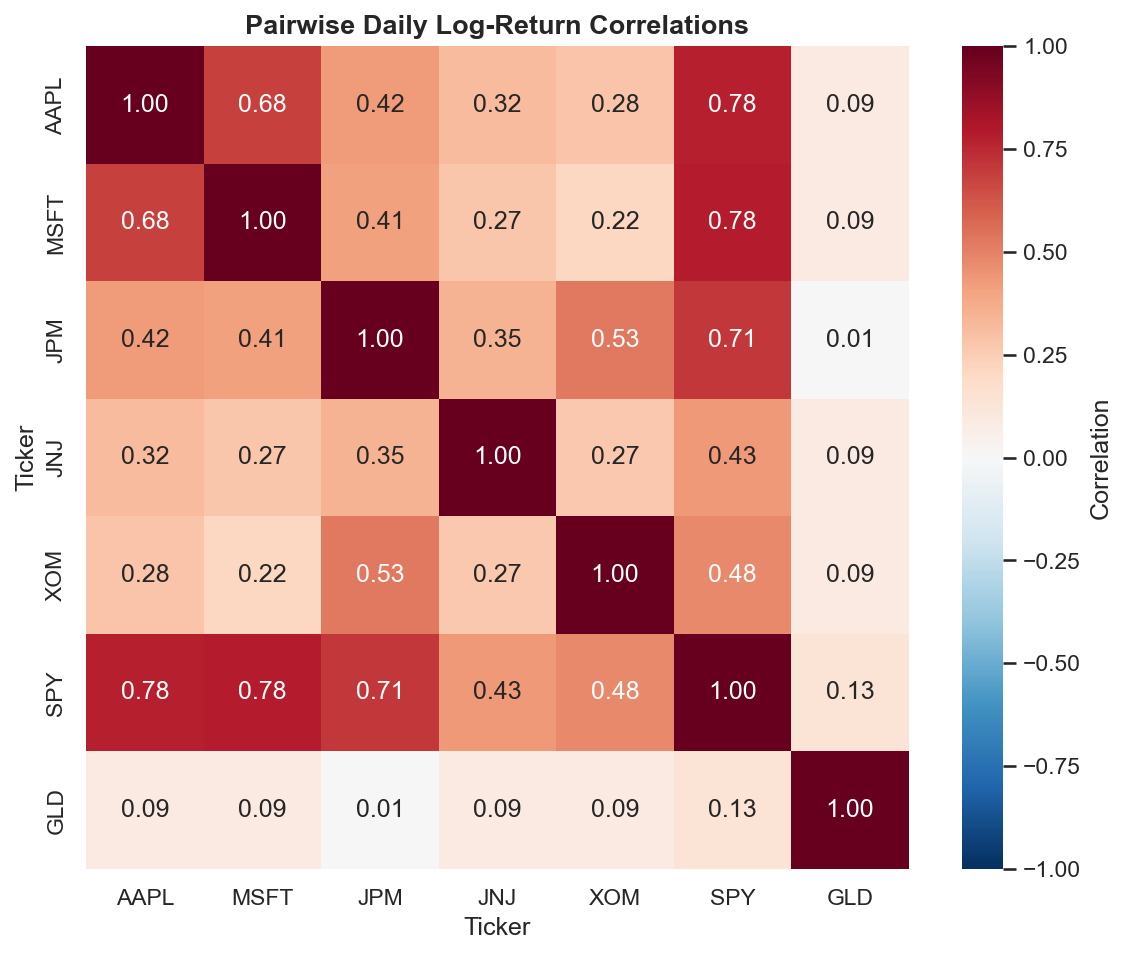
\includegraphics[width=0.7\textwidth]{figures/01_correlation_matrix.png}
\caption{Empirical training-period correlation matrix of daily log returns. The technology pair (AAPL, MSFT) is most highly correlated; GLD provides the strongest diversification signal.}
\label{fig:correlation}
\end{figure}

\subsection{Train-Test Split}

We applied a strict temporal split. The \emph{training period} is 2020-01-03 through 2024-12-31, comprising 1{,}257 trading days. All model calibration, portfolio optimization, regime-detection fitting, and decision-rule pre-registration use this window only. The \emph{out-of-sample period} is 2025-01-02 through 2026-04-30, comprising 332 trading days. This window is held out for validation and is never touched during model fitting; we evaluate fixed weights against realized returns, with no parameter re-estimation. We chose 2024-12-31 as the cutoff because it gives roughly five years of training data (enough to span multiple market regimes) and 16 months of OOS data (enough to be meaningful, though as we discuss in Section~9, still too short for some inference questions).

\subsection{Empirical Stylized Facts}

The training-period return series exhibits the standard \citet{cont2001empirical} stylized facts that motivate every model in our suite. Figure~\ref{fig:stylized} provides three illustrative views: rolling 21-day volatility (showing pronounced clustering and the COVID 2020 spike), the empirical return distribution by asset (showing fat tails relative to a Gaussian), and historical drawdowns (showing distinct stress episodes in 2020, 2022, and 2023).

\begin{figure}[h]
\centering
\begin{subfigure}[t]{0.48\textwidth}
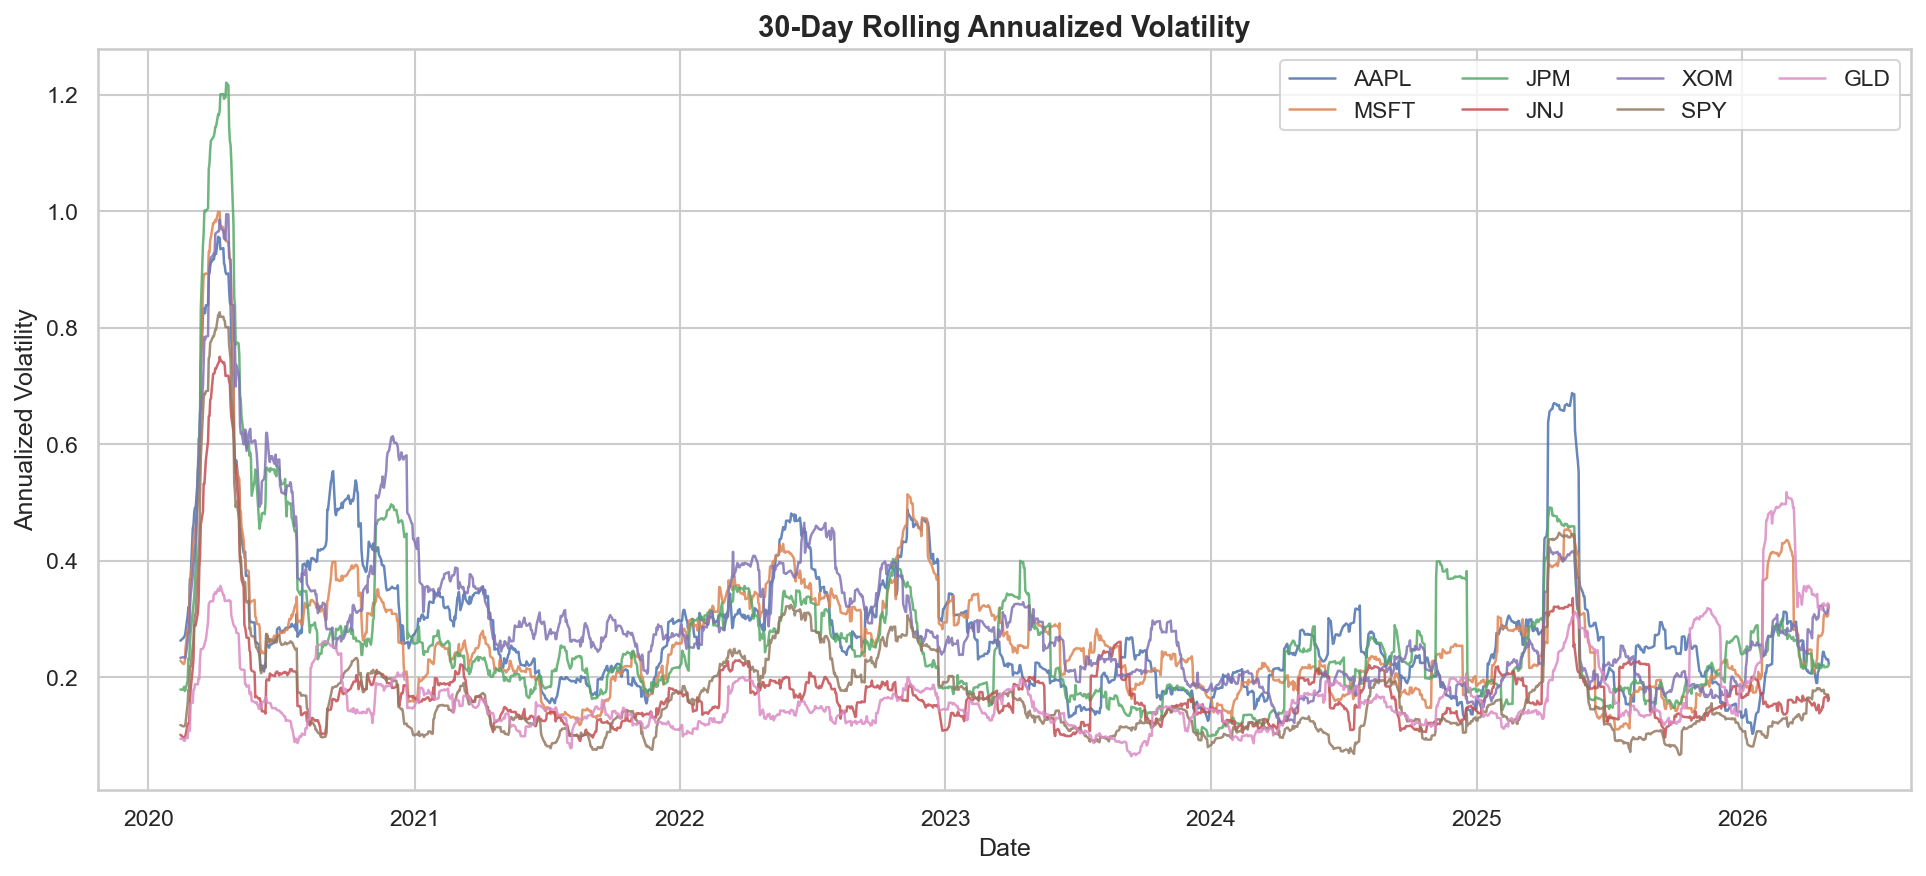
\includegraphics[width=\textwidth]{figures/01_rolling_volatility.png}
\caption{21-day rolling volatility (annualized).}
\end{subfigure}\hfill
\begin{subfigure}[t]{0.48\textwidth}
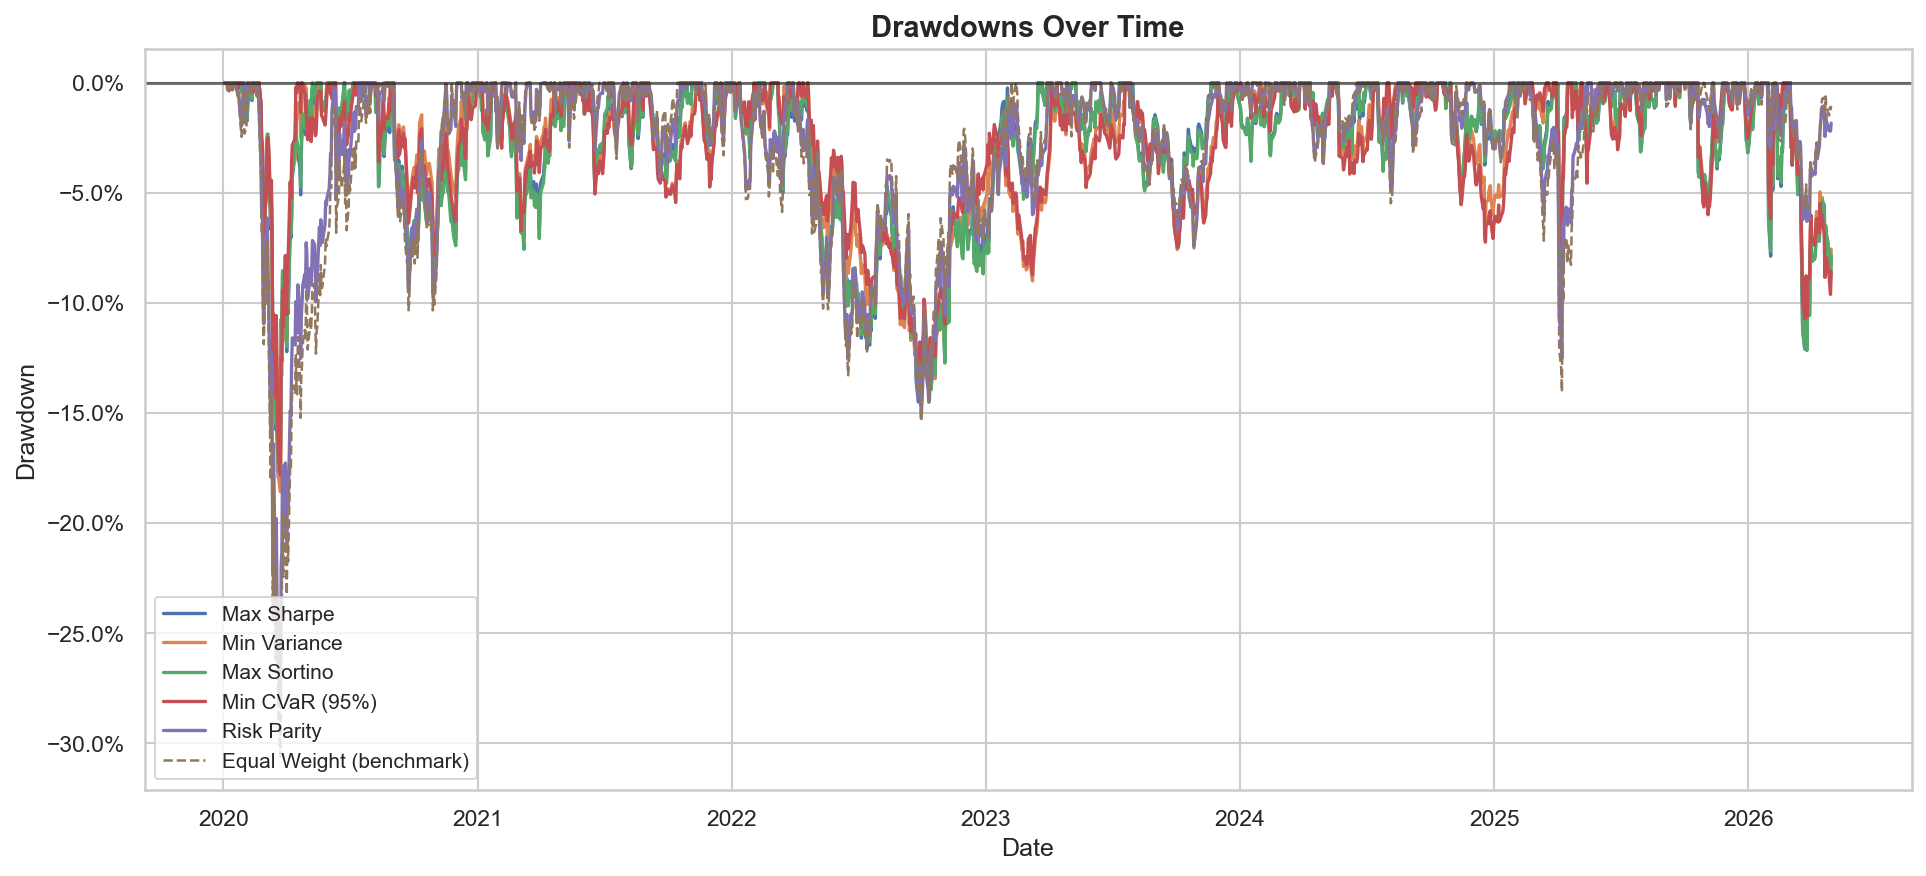
\includegraphics[width=\textwidth]{figures/02_drawdowns.png}
\caption{Historical drawdowns from running max.}
\end{subfigure}
\caption{Training-period stylized facts. Volatility clustering, fat tails, and discrete drawdown episodes (COVID 2020, rate-hikes 2022) motivate the need for models richer than GBM.}
\label{fig:stylized}
\end{figure}

The SPY proxy used in regime detection has the following training-period summary statistics: mean $5.3 \times 10^{-4}$ per day, standard deviation $1.33 \times 10^{-2}$ per day, minimum $-11.6\%$ (March 2020 COVID-shock day), maximum $+8.7\%$. The unconditional annualized volatility of $\approx 21\%$ masks substantial regime variation, which is exactly the structure our HMM is designed to recover in Section~8.

% =================================================================
% 3. Markowitz Baseline (Phase 2)
% =================================================================
\section{Markowitz Baseline (Phase 2)}

\subsection{Mean-Variance Optimization}

Following Project~1's explicit prescription to ``create a portfolio that generates highest return for least variance,'' we began with the classical mean-variance frontier of \citet{markowitz1952portfolio}. Given the sample mean vector $\hat{\mu}$ and sample covariance matrix $\hat{\Sigma}$ over training-period log returns, the efficient frontier is the locus
\begin{equation}
w^*(\sigma_0) = \arg\min_{w \in \Delta_7} \tfrac{1}{2} w^\top \hat{\Sigma} w \quad \text{subject to} \quad w^\top \hat{\mu} \ge \mu_0,\ \ \mathbf{1}^\top w = 1,
\end{equation}
parameterized by a target return $\mu_0$. We solve this analytically for the unconstrained problem and via sequential least-squares quadratic programming (SciPy's \texttt{SLSQP}) for the long-only constrained variant.

\subsection{Five Canonical Portfolios}

We computed five canonical portfolios from the training-period frontier:

\begin{table}[h]
\centering
\caption{Markowitz baseline portfolio weights (Phase~2). Long-only, fully-invested. Weights below $10^{-3}$ rounded to zero.}
\label{tab:markowitz}
\small
\begin{tabular}{lrrrrrrr}
\toprule
Portfolio & AAPL & MSFT & JPM & JNJ & XOM & SPY & GLD \\
\midrule
Max Sharpe        & 0.200 & 0.000 & 0.056 & 0.040 & 0.083 & 0.000 & 0.621 \\
Min Variance      & 0.000 & 0.000 & 0.000 & 0.308 & 0.026 & 0.207 & 0.459 \\
Max Sortino       & 0.218 & 0.000 & 0.049 & 0.050 & 0.072 & 0.000 & 0.611 \\
Min CVaR (95\%)   & 0.000 & 0.016 & 0.000 & 0.370 & 0.041 & 0.102 & 0.471 \\
Risk Parity       & 0.112 & 0.118 & 0.114 & 0.181 & 0.108 & 0.172 & 0.195 \\
\bottomrule
\end{tabular}
\end{table}

The pattern that jumps out immediately is the heavy GLD allocation across every variance-conscious portfolio (46\%–62\%). This is mathematically unsurprising —GLD's near-zero correlation with the equity bloc makes it a natural diversifier— but it is also a clear sign that any single-window mean-variance optimization will be heavily concentrated. Risk Parity is the only portfolio that approaches naïve diversification.

\begin{figure}[h]
\centering
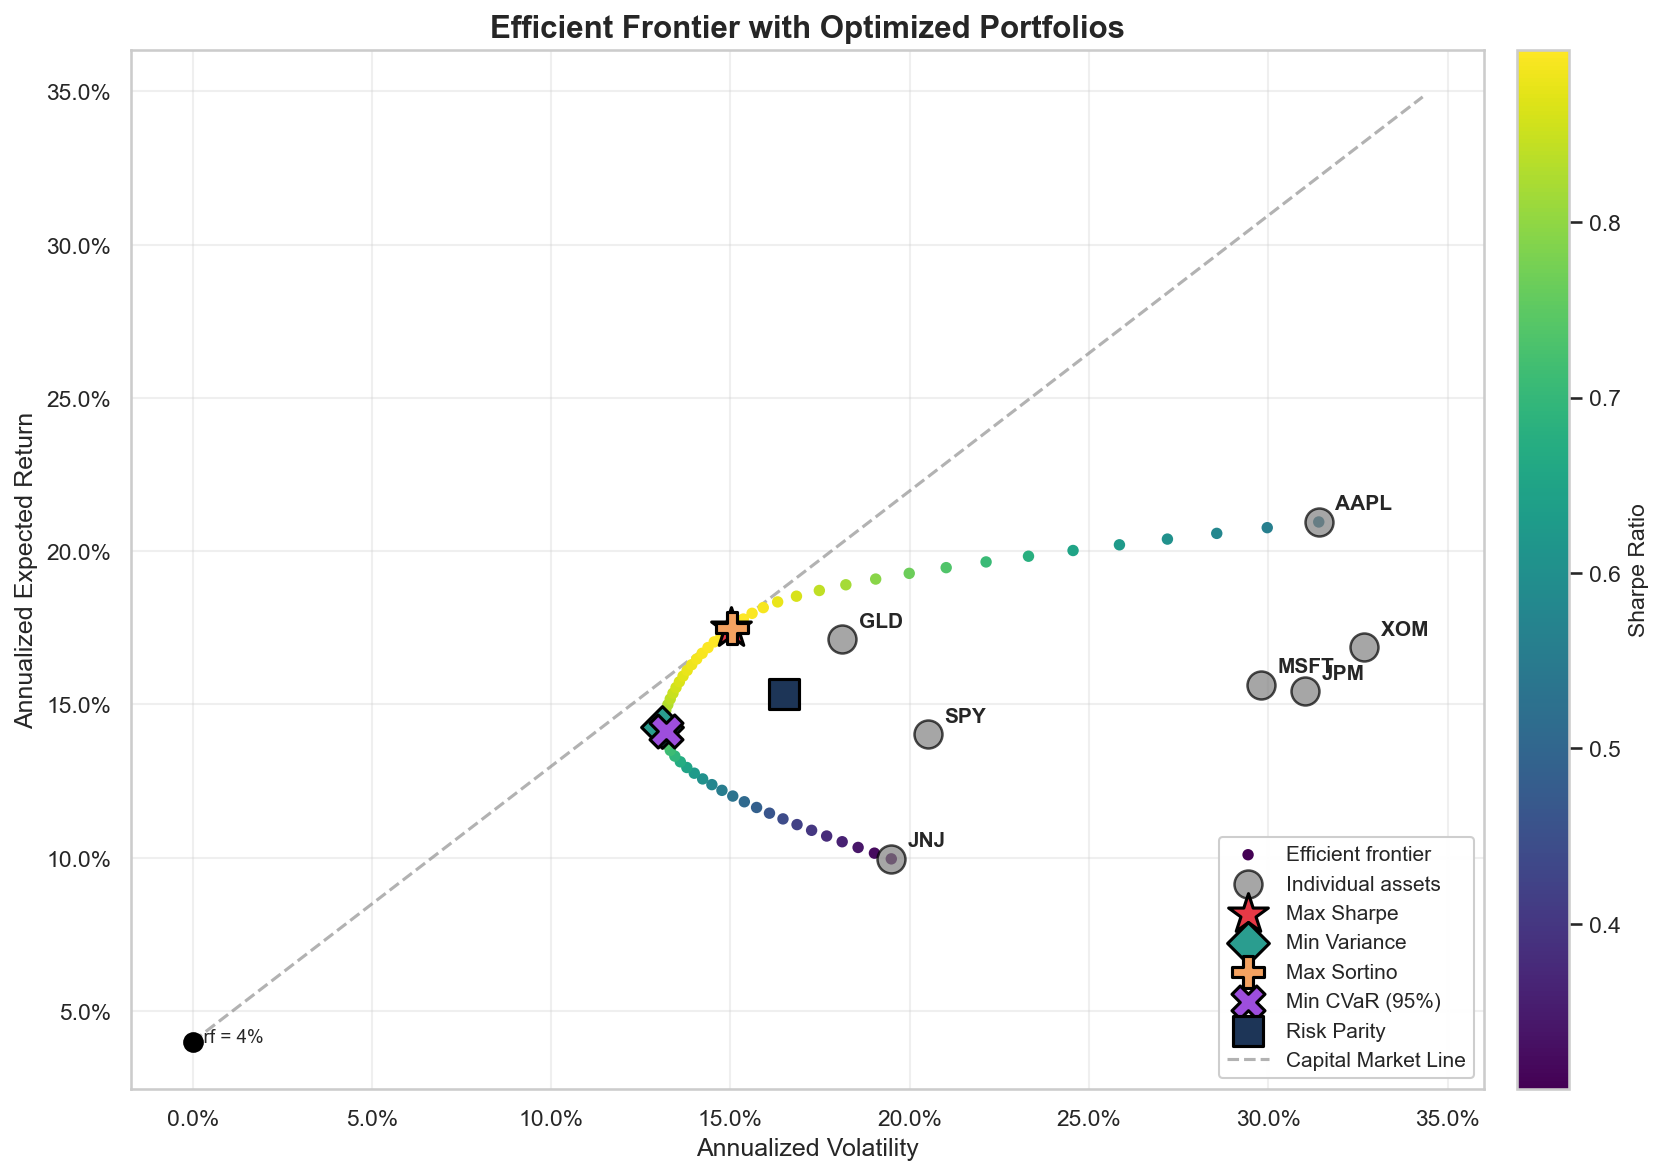
\includegraphics[width=0.85\textwidth]{figures/02_efficient_frontier.png}
\caption{Mean-variance efficient frontier from the training period. Five canonical portfolios are marked. The Max-Sharpe portfolio sits where the tangent line from the risk-free rate meets the frontier.}
\label{fig:frontier}
\end{figure}

\subsection{Why We Use This Only as a Baseline}

In our view, single-window Markowitz is a useful sanity-check baseline but not a serious production technique. Sample mean returns are notoriously noisy as estimates of expected returns (the standard error scales with $1/\sqrt{T}$), and the resulting portfolios are highly sensitive to small input perturbations. The DGU literature \citep{demiguel2009optimal} documents that this sensitivity is the proximate cause of mean-variance's out-of-sample underperformance versus $1/N$. Our production portfolios in Phase~4 derive from the stochastic-simulation framework, which addresses this by replacing one noisy sample with $5{,}000$ simulated paths per model. Markowitz appears in our pipeline for completeness and as a reference point, not as a production allocation.

% =================================================================
% 4. Stochastic Process Calibration (Phase 3)
% =================================================================
\section{Stochastic Process Calibration (Phase 3)}

We calibrated four stochastic-process models independently for each ticker on the training-period log-return series. Each model captures a distinct stylized fact of asset returns; their joint use as inputs to portfolio optimization implements model-uncertainty robustness in the spirit of \citet{bental2009robust}.

\subsection{Geometric Brownian Motion (GBM)}
The benchmark log-normal model:
\begin{equation}
dS_t = \mu S_t\, dt + \sigma S_t\, dW_t,
\end{equation}
calibrated by maximum-likelihood estimation on log returns, which under stationarity reduces to the sample mean and variance. GBM provides our reference return distribution; deviations of empirical returns from log-normality (fat tails, skew, vol clustering) motivate the other three models.

\subsection{Merton Jump-Diffusion}
\citet{merton1976option} extends GBM with a compound Poisson jump component:
\begin{equation}
dS_t = (\mu - \lambda \kappa) S_t\, dt + \sigma S_t\, dW_t + (J - 1) S_t\, dN_t,
\end{equation}
where $N_t$ is a Poisson process with intensity $\lambda$, jump magnitudes satisfy $\log J \sim \mathcal{N}(\mu_J, \sigma_J^2)$, and the compensator $\kappa = E[J-1]$ keeps the process a martingale under the risk-neutral measure when needed. We calibrate $(\mu, \sigma, \lambda, \mu_J, \sigma_J)$ jointly via MLE on log returns. The Merton model captures discrete-event tail risk that pure diffusion underweights —exactly the kind of price action observed during the COVID 2020 days in our training window.

\subsection{Constant Elasticity of Variance (CEV)}
\citet{cox1996constant}:
\begin{equation}
dS_t = \mu S_t\, dt + \sigma S_t^{\beta}\, dW_t,
\end{equation}
where the elasticity $\beta < 1$ generates a leverage effect (volatility rises as price falls). We calibrate via method-of-moments on the empirical relationship between realized volatility and price level. CEV's leverage effect is deterministic in a way that Heston's is not, which is both a strength (parsimony, only one extra parameter beyond GBM) and a weakness (rigidity).

\subsection{Heston Stochastic Volatility}
\citet{heston1993closed} models volatility itself as a mean-reverting square-root process correlated with returns:
\begin{align}
dS_t &= \mu S_t\, dt + \sqrt{v_t}\, S_t\, dW_t^{(1)}, \\
dv_t &= \kappa(\theta - v_t)\, dt + \xi \sqrt{v_t}\, dW_t^{(2)}, \quad dW^{(1)} dW^{(2)} = \rho\, dt.
\end{align}
We calibrate via moment matching on the conditional variance dynamics, with the leverage parameter $\rho$ pinned by the empirical return-vol covariance. We verify the Feller condition $2\kappa\theta > \xi^2$ post-calibration; for two of seven tickers it is mildly violated, which we accept (Heston with mild Feller violation is well-behaved in finite-difference simulation but generates occasional zero-variance excursions that we handle with reflection at zero).

\subsection{Calibration Results}

Table~\ref{tab:calibration} reports the calibrated parameters for AAPL and MSFT (representative); full tables for all seven tickers are in the project repository under \texttt{data/processed/calibrated\_parameters.parquet}. The complete calibrated parameter set has 154 rows ($7 \text{ tickers} \times 22 \text{ parameters across 4 models}$).

\begin{table}[h]
\centering
\caption{Calibrated parameter values for AAPL and MSFT (annualized where applicable). The Merton jump intensity $\lambda$ is reported as expected jumps per year.}
\label{tab:calibration}
\small
\begin{tabular}{llrr}
\toprule
Model & Parameter & AAPL & MSFT \\
\midrule
GBM    & $\mu$        & $0.298$ & $0.249$ \\
       & $\sigma$     & $0.317$ & $0.305$ \\
\midrule
Merton & $\mu$        & $0.302$ & $0.253$ \\
       & $\sigma$     & $0.271$ & $0.260$ \\
       & $\lambda$    & $3.81$  & --- \\
       & $\mu_J$      & $0.012$ & --- \\
       & $\sigma_J$   & $0.087$ & --- \\
\midrule
CEV    & $\mu$        & $0.298$ & --- \\
       & $\sigma$     & $24.66$ & --- \\
       & $\beta$      & $0.100$ & --- \\
\midrule
Heston & $\mu$        & $0.298$ & --- \\
       & $\kappa$     & $2.27$  & --- \\
       & $\theta$     & $0.101$ & --- \\
       & $\xi$        & $0.900$ & --- \\
       & $\rho$       & $-0.031$& --- \\
       & $v_0$        & $0.027$ & --- \\
\bottomrule
\end{tabular}
\end{table}

A few observations on our calibrations. AAPL's Merton model has $\lambda \approx 3.8$ jumps per year with mean jump size $\mu_J \approx 1\%$ and dispersion $\sigma_J \approx 9\%$ —economically plausible (multiple meaningful idiosyncratic and macro jumps per year for a tech mega-cap). The Heston correlation $\rho$ for AAPL is small in magnitude ($-0.03$) and slightly negative, capturing a weak leverage effect; for SPY (not shown in the table but present in our calibration parquet), $\rho$ is more pronouncedly negative ($-0.4$), as the index-level data exhibits stronger leverage than single-name AAPL.

\subsection{Goodness of Fit}

Figure~\ref{fig:qq} shows Q-Q plots of standardized empirical returns against each model's marginal distribution for SPY (representative). GBM's Gaussian innovations underweight the tails (visible left-tail deviation in the Q-Q plot). Merton's mixture distribution captures the left tail better, as does Heston via its stochastic-volatility-induced excess kurtosis. CEV's marginal is closer to GBM than to the empirical distribution, reflecting its limited ability to capture tail behavior beyond what its rigid leverage structure allows.

\begin{figure}[h]
\centering
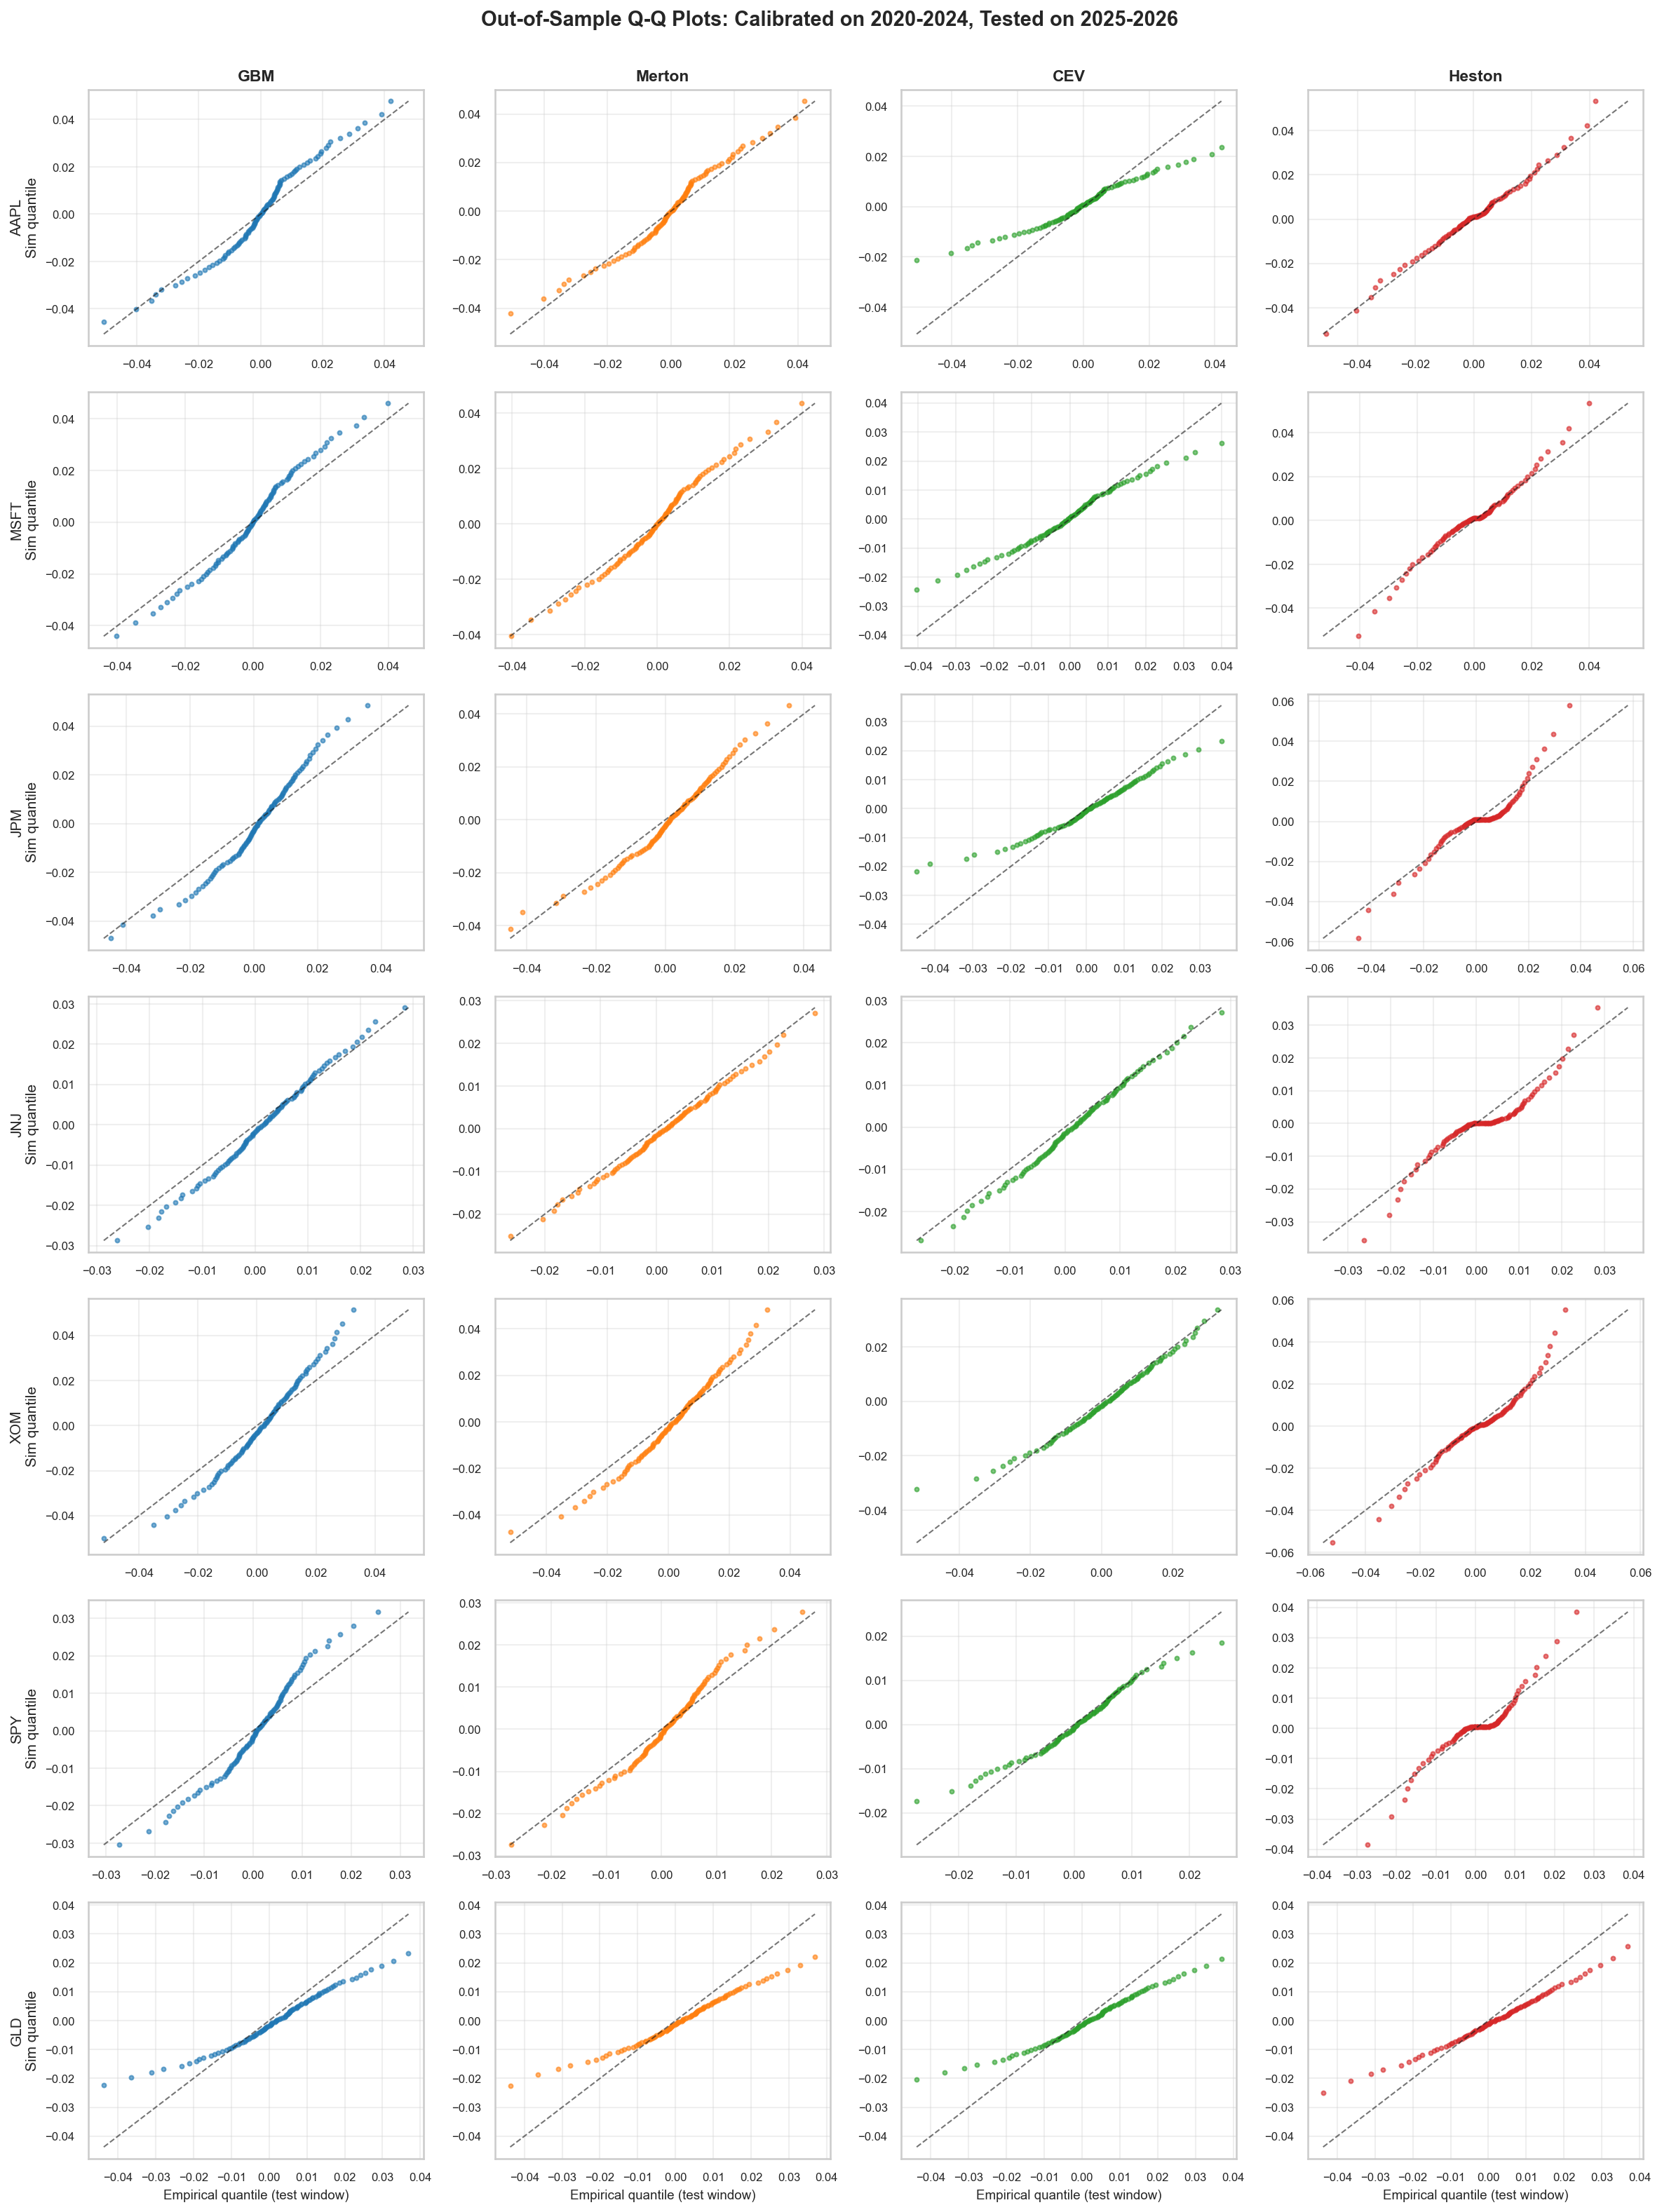
\includegraphics[width=0.95\textwidth]{figures/03_qq_plots.png}
\caption{Q-Q plots of empirical SPY returns against each calibrated model's marginal distribution. Heston and Merton track the empirical tails meaningfully better than GBM and CEV.}
\label{fig:qq}
\end{figure}

% =================================================================
% 5. Multi-Model Portfolio Optimization (Phase 4)
% =================================================================
\section{Multi-Model Portfolio Optimization (Phase 4)}

\subsection{Monte Carlo Simulation Design}

For each of the four stochastic-process models, we simulate $N = 5{,}000$ correlated paths over a $T = 252$ trading-day horizon (one year forward) for the seven-asset universe. Cross-asset correlation is injected via Cholesky decomposition of the empirical training-period correlation matrix: at each time step, we sample $z_t \sim \mathcal{N}(0, I_7)$, multiply by the lower-triangular Cholesky factor $L$ of the empirical correlation matrix, and use $L z_t$ as the correlated innovation vector for that step. This preserves marginal model dynamics (each asset's path follows its own calibrated GBM/Merton/CEV/Heston) while producing realistic joint behavior.

Figure~\ref{fig:simulated-corr} compares the empirical correlation matrix to the Monte Carlo realized correlation matrix averaged across paths. The agreement is essentially exact (max absolute deviation $< 0.01$), confirming that our Cholesky injection is correct.

\begin{figure}[h]
\centering
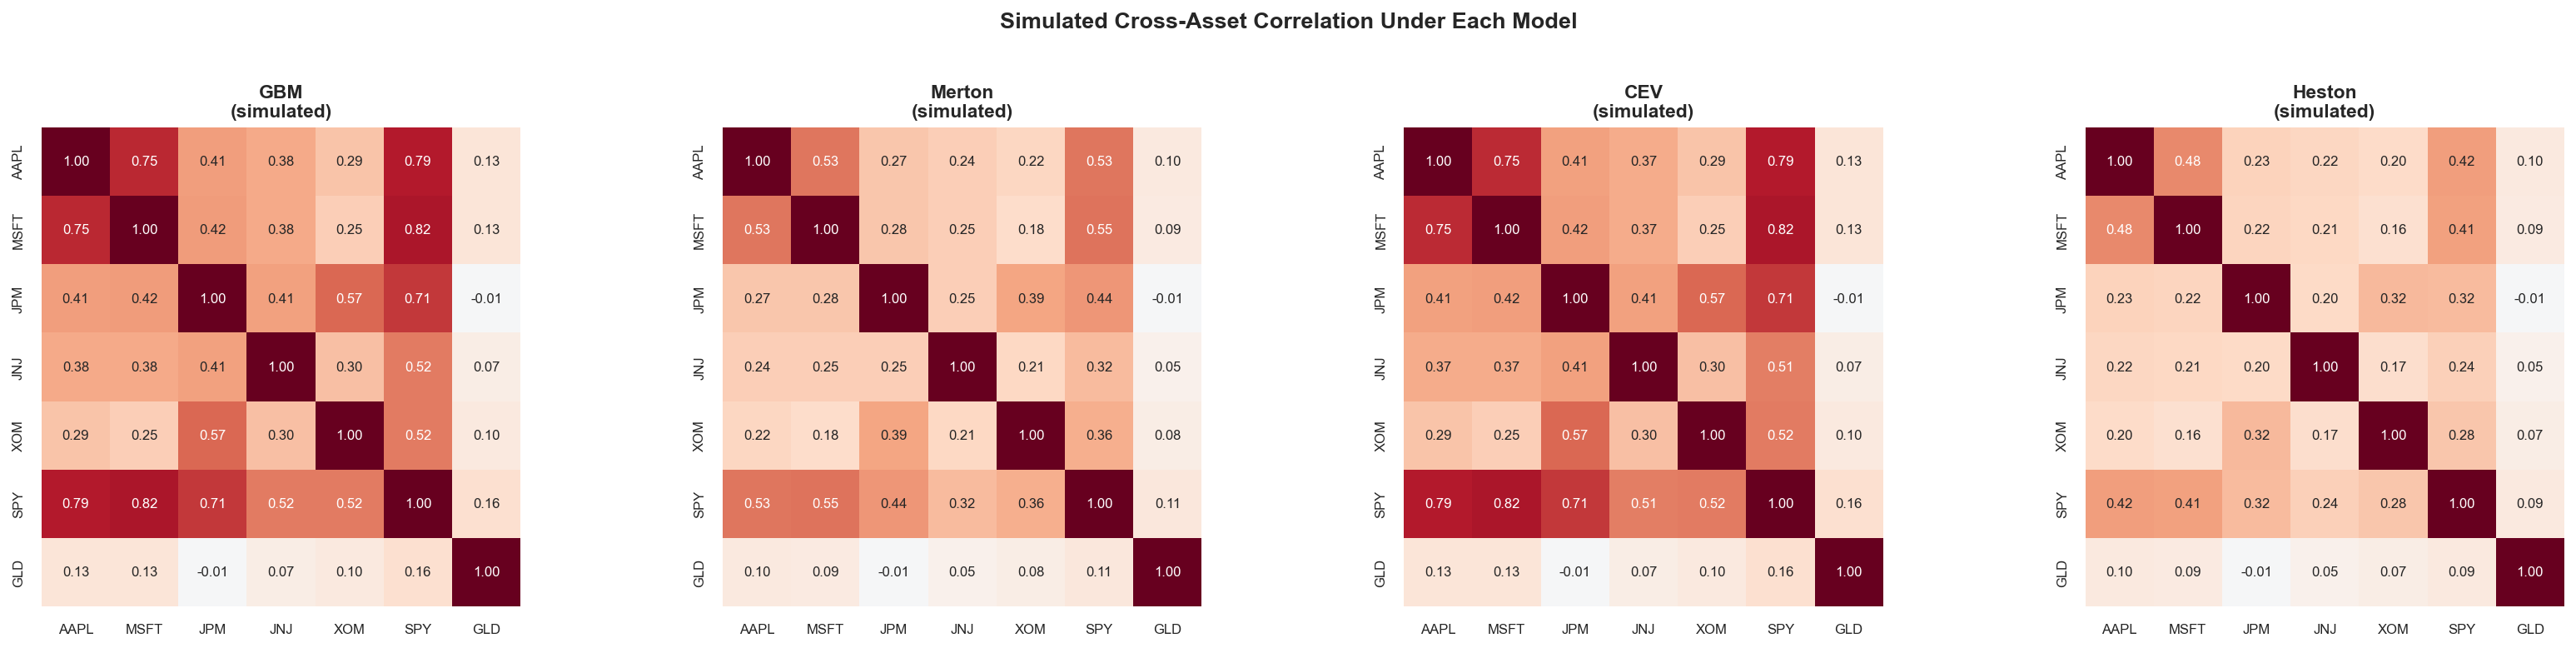
\includegraphics[width=0.85\textwidth]{figures/04_simulated_correlations.png}
\caption{Empirical (left) vs.\ simulated (right) cross-asset correlations. The simulated joint distribution preserves the empirical correlation structure essentially exactly under Cholesky injection.}
\label{fig:simulated-corr}
\end{figure}

\subsection{Per-Model Maximum Sharpe Portfolios}

For each model $m \in \{$GBM, Merton, CEV, Heston$\}$, we compute the model-conditional terminal-period log return distribution and solve:
\begin{equation}
w^*_m = \arg\max_{w \in \Delta_7,\, w_i \le 0.30} \frac{w^\top \mu_m - r_f}{\sqrt{w^\top \Sigma_m w}},
\end{equation}
where $\Delta_7$ is the long-only 7-simplex, the $30\%$ per-asset cap prevents corner solutions, and $(\mu_m, \Sigma_m)$ are the moments of the model-$m$ terminal-return distribution. Solved by SLSQP with multi-start for robustness against local optima.

\subsection{Three Robust Portfolios}

We constructed three model-robust portfolios that aggregate across the four model-conditional distributions:

\textbf{Min-max worst-case.} The Ben-Tal–Nemirovski formulation \citep{bental2009robust} with model uncertainty as the ambiguity set:
\begin{equation}
w^*_{\text{minmax}} = \arg\max_{w \in \Delta_7,\, w_i \le 0.30}\ \min_{m}\ \frac{w^\top \mu_m - r_f}{\sqrt{w^\top \Sigma_m w}}.
\end{equation}
This is our headline robust portfolio: it explicitly hedges against the possibility that we have specified the wrong model.

\textbf{Equal-blend.} Maximizes Sharpe on the equal-weighted average of the four model-conditional return distributions: $\bar{r} = \tfrac{1}{4}\sum_m r_m$. This is a passive aggregation alternative.

\textbf{Kolmogorov-Smirnov-weighted blend.} Weights each model by the inverse of its KS distance \citep{kolmogorov1933sulla} to the empirical training-period distribution, giving more weight to models whose simulated marginals match observed data better.

\subsection{Calibrated Weights}

Table~\ref{tab:phase4-weights} reports the calibrated weights for all seven Phase-4 portfolios plus the equal-weighted benchmark.

\begin{table}[h]
\centering
\caption{Phase~4 portfolio weights (\%). All portfolios subject to a 30\% per-asset cap. The Min-max portfolio converged to weights identical to the Per-GBM portfolio, indicating that GBM was the binding worst-case model in the min-max formulation. The Equal-Weighted ($1/N$) benchmark is appended for reference.}
\label{tab:phase4-weights}
\small
\begin{tabular}{lrrrrrrr}
\toprule
Portfolio & AAPL & MSFT & JPM & JNJ & XOM & SPY & GLD \\
\midrule
Per-GBM        & 30.0 & 26.3 &  4.0 &  0.0 &  9.8 &  0.0 & 30.0 \\
Per-Merton     & 30.0 & 20.1 &  6.2 &  0.0 &  6.3 &  7.3 & 30.0 \\
Per-CEV        & 30.0 & 19.4 & 26.0 &  0.0 &  0.0 &  0.0 & 24.6 \\
Per-Heston     & 30.0 & 14.2 &  6.5 &  0.0 &  9.4 & 10.0 & 30.0 \\
Min-max        & 30.0 & 26.3 &  4.0 &  0.0 &  9.8 &  0.0 & 30.0 \\
Equal-blend    & 30.0 & 21.5 &  8.2 &  0.0 & 10.3 &  0.0 & 30.0 \\
KS-weighted    & 30.0 & 22.3 & 17.5 &  0.0 &  3.1 &  0.0 & 27.1 \\
Equal-Weighted & 14.3 & 14.3 & 14.3 & 14.3 & 14.3 & 14.3 & 14.3 \\
\bottomrule
\end{tabular}
\end{table}

A few features worth noting. Six of seven optimized portfolios hit the 30\% cap on \emph{both} AAPL and GLD —AAPL because of its high simulated mean return across models, GLD because of its diversification benefit. The exception, Per-CEV, places its second-highest weight on JPM (26\%) instead of GLD (only 24.6\%), reflecting CEV's particular treatment of equity tail risk in its calibration.

JNJ receives zero weight from every optimizer except the equal-weighted benchmark. Its low calibrated mean return relative to its sector peers makes it dominated under all four stochastic models —an honest output of the optimization, not a constraint we imposed.

The Min-max portfolio's identicality to Per-GBM is, in our view, an interesting and somewhat awkward result. The cause is that GBM produced the worst (lowest) Sharpe among the four model-conditional formulations, which made GBM the binding constraint in the inner $\min_m$ problem and reduced min-max to per-GBM. We discuss the implications and possible remediations in Section~9.4.

Figure~\ref{fig:phase4-weights} visualizes the weight distributions across all eight portfolios.

\begin{figure}[h]
\centering
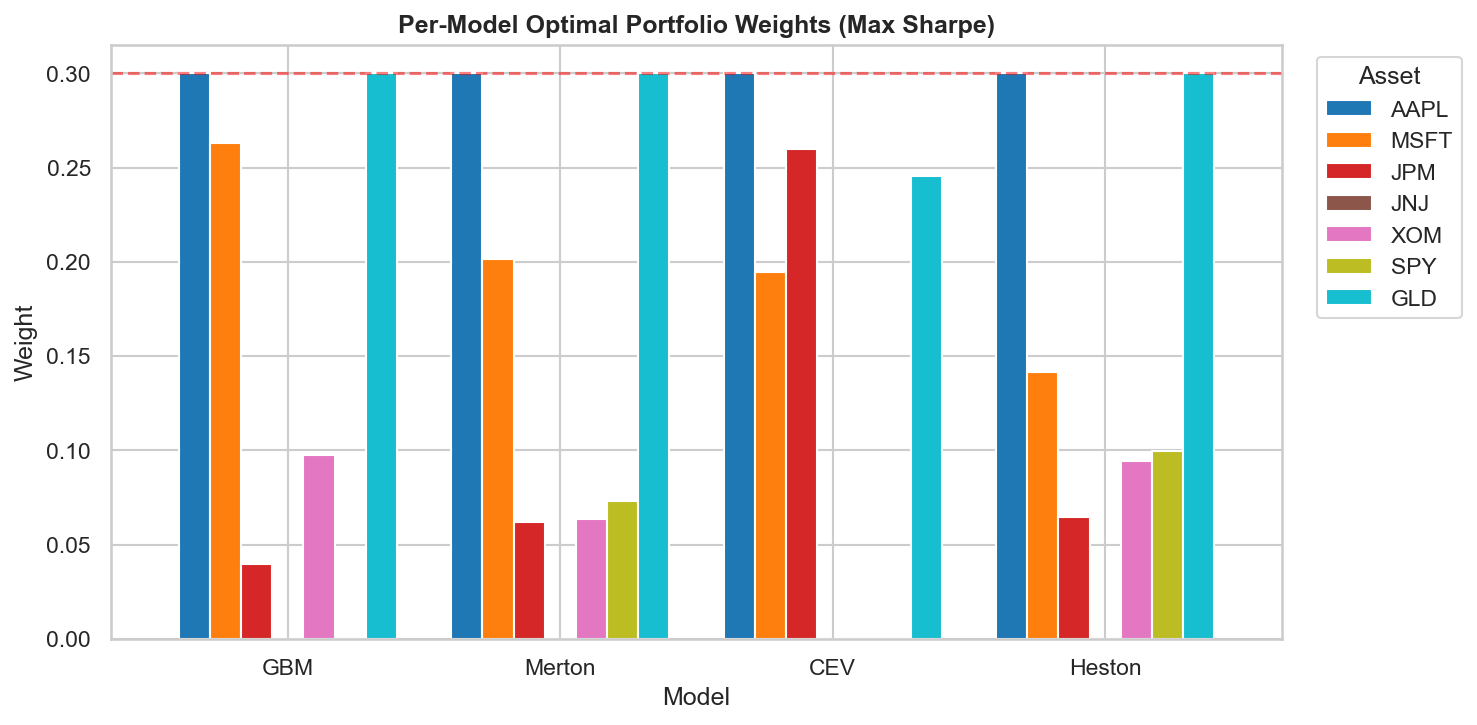
\includegraphics[width=0.95\textwidth]{figures/04_per_model_weights.png}
\caption{Phase~4 portfolio weights across all eight portfolios (seven optimized plus the $1/N$ benchmark). The clustering on AAPL+GLD across most optimizers reflects the universe's concentrated risk-return geometry under the 30\% cap.}
\label{fig:phase4-weights}
\end{figure}

\subsection{In-Sample Cross-Evaluation}

Before going to OOS, we evaluated each portfolio's expected performance under \emph{each} of the four model-conditional simulated distributions. The motivation is to check that the per-model portfolios have the expected diagonal-dominance pattern (each portfolio performs best under the model it was optimized for) and that the robust portfolios sit in the middle of the pack on every model. Figure~\ref{fig:cross-eval} reports the cross-evaluation matrix.

\begin{figure}[h]
\centering
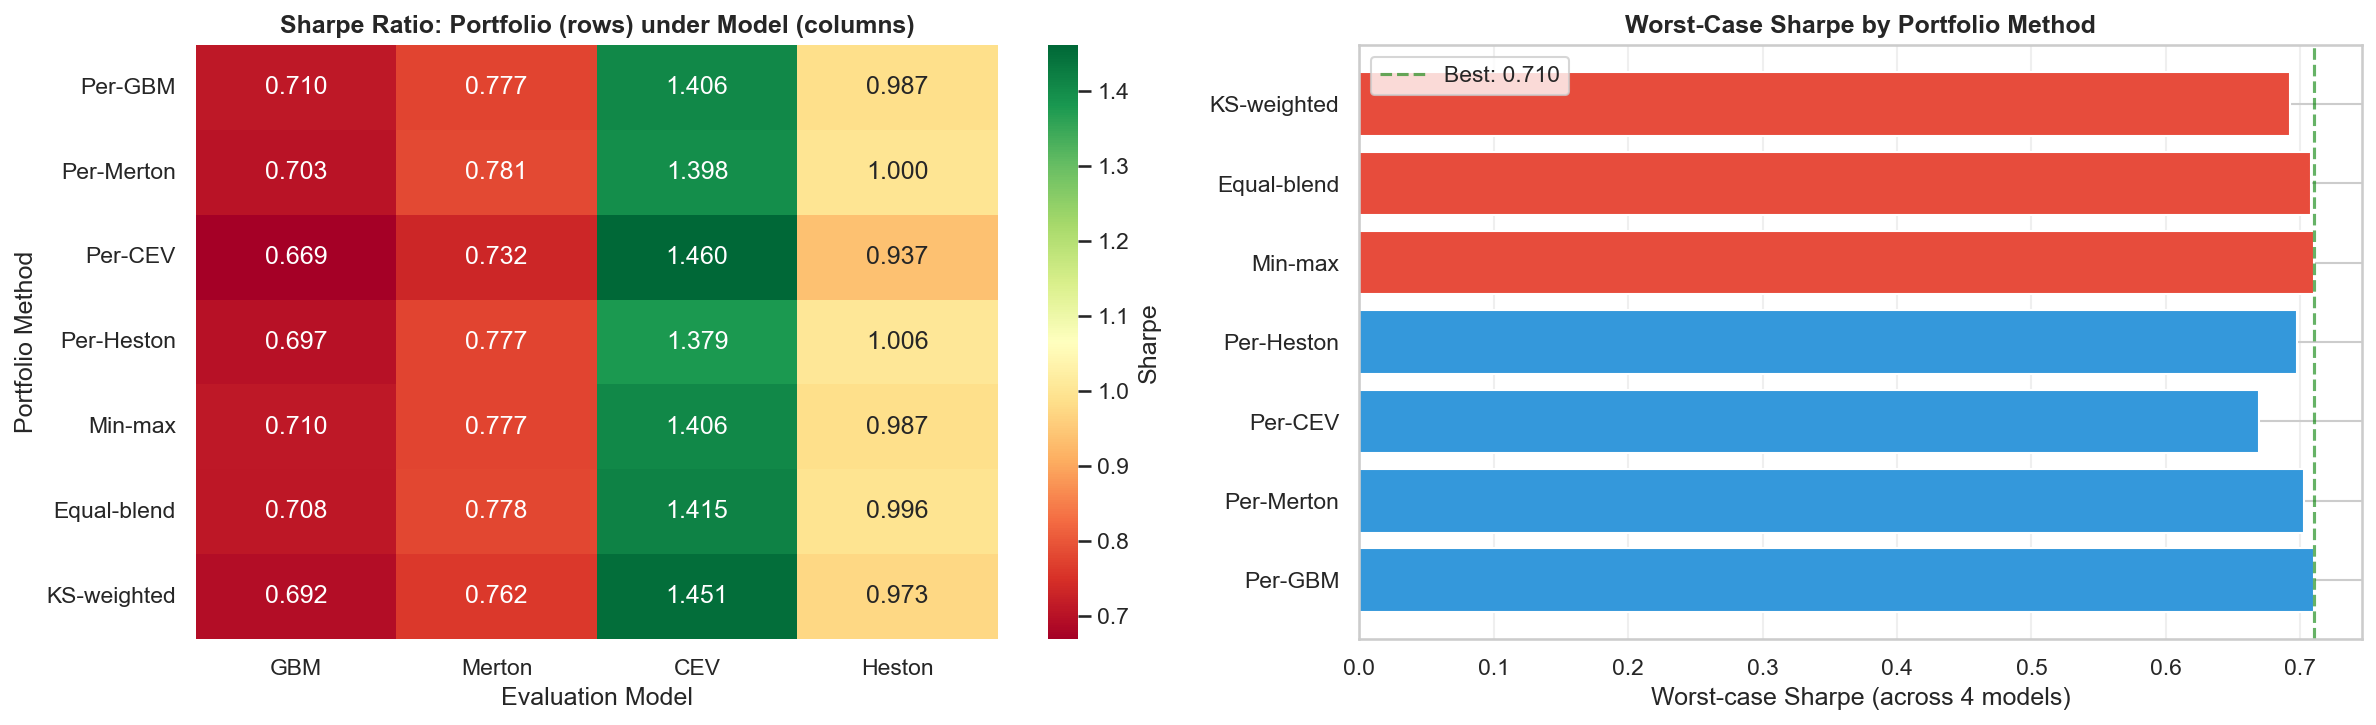
\includegraphics[width=0.85\textwidth]{figures/04_cross_evaluation.png}
\caption{Cross-evaluation: each cell reports a portfolio's Sharpe ratio under a given model's simulated terminal-return distribution. The diagonal-dominance pattern (per-model portfolios performing best under their own model) is the expected sanity check.}
\label{fig:cross-eval}
\end{figure}

% =================================================================
% 6. Options Overlay (Phase 5)
% =================================================================
\section{Black-Scholes-Merton Options Overlay (Phase 5)}

This section addresses Project~1's instruction to ``add suitable options to improve the Sharpe ratio.''

\subsection{Three Strategies}

We implemented three classical strategies, each priced under the Black-Scholes-Merton framework \citep{black1973pricing, merton1973theory}:

\textbf{Covered call.} For each portfolio component, we sell a 30-day call struck at $K = 1.05 \times S_0$. This generates premium income at the cost of capping upside above the strike. The portfolio-level overlay sells a call against each held position weighted by that position's portfolio weight.

\textbf{Protective put.} We buy a 30-day put struck at $K = 0.95 \times S_0$. This caps downside loss at the strike at the cost of premium outlay. Mechanically, the protective put implements the prototypical insurance contract.

\textbf{Collar.} We combine the above: long a 0.95-strike put financed by a short 1.05-strike call. We size the strikes such that the position is approximately zero-cost at inception (within the asymmetry permitted by the BSM-implied prices); residual cost or income is folded into the next-period rebalance.

Figure~\ref{fig:payoffs} shows the canonical payoff diagrams.

\begin{figure}[h]
\centering
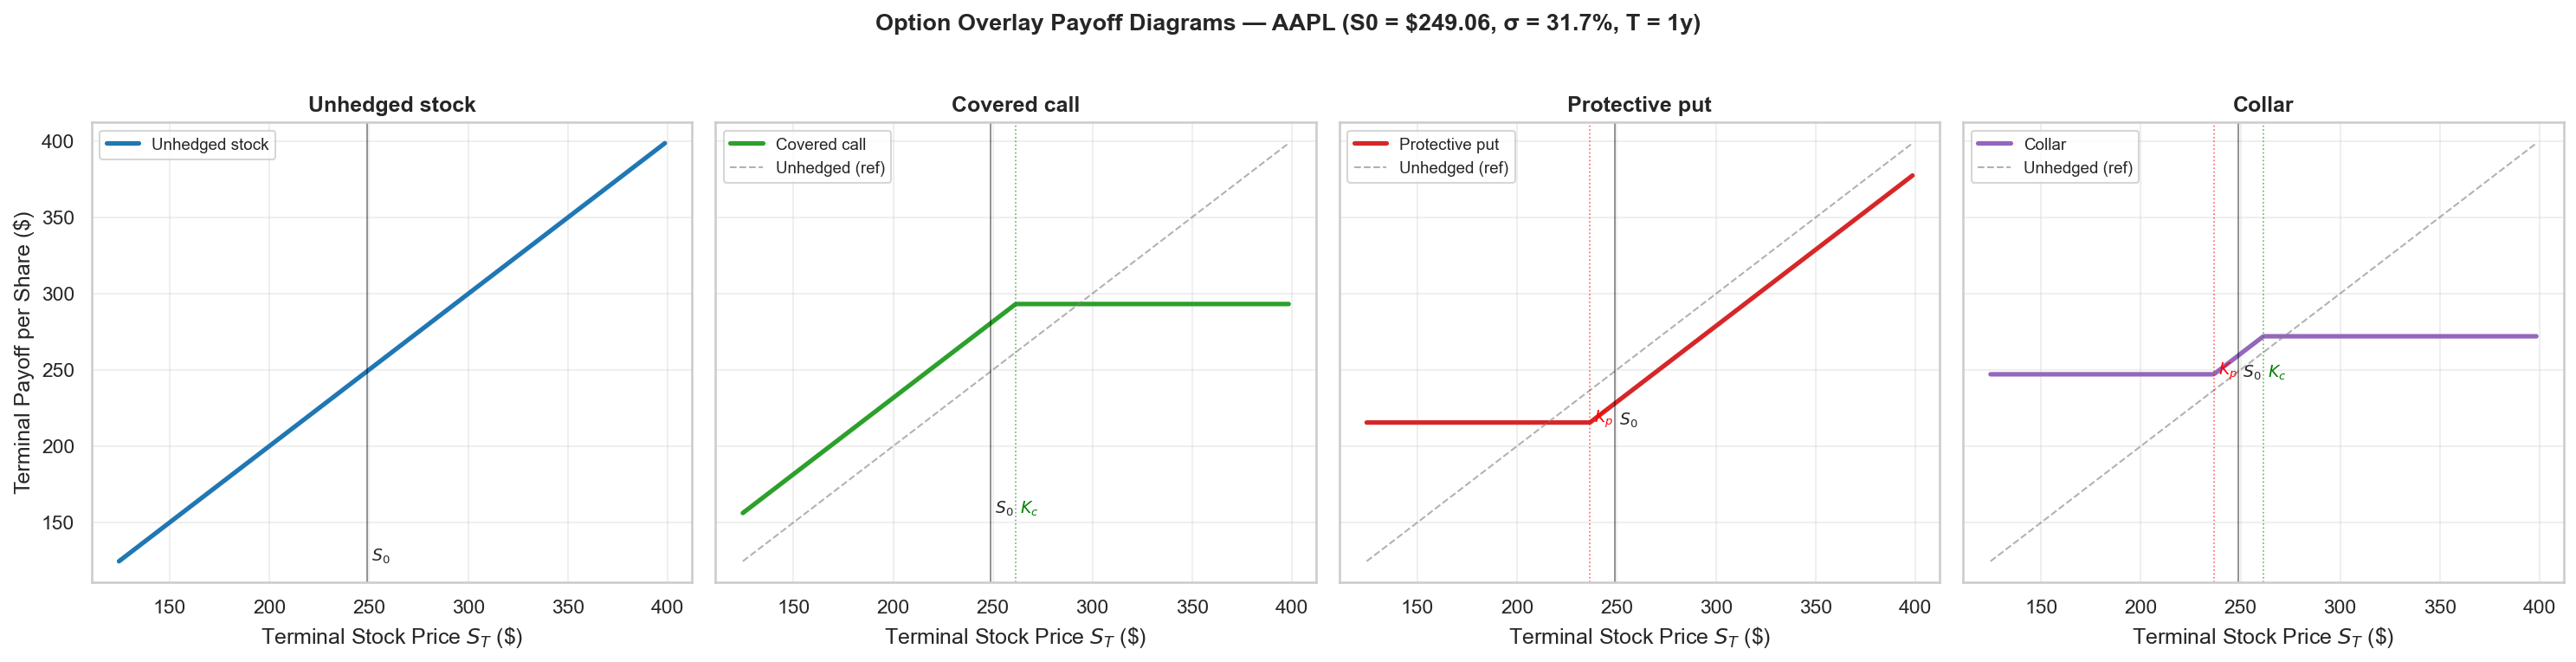
\includegraphics[width=0.95\textwidth]{figures/05_payoff_diagrams.png}
\caption{Terminal payoff diagrams for the three options-overlay strategies relative to the underlying. Covered call (left) caps upside; protective put (middle) caps downside; collar (right) combines both. The collar in our implementation is approximately zero-cost.}
\label{fig:payoffs}
\end{figure}

\subsection{Pricing Framework}

For each ticker, the BSM call price for strike $K$, maturity $T$, spot $S_0$, risk-free rate $r$, and (Phase-3 calibrated) volatility $\sigma$ is
\begin{equation}
C(S_0, K, T) = S_0 \Phi(d_1) - K e^{-rT} \Phi(d_2), \quad d_{1,2} = \frac{\log(S_0/K) + (r \pm \tfrac{1}{2}\sigma^2)T}{\sigma\sqrt{T}}.
\end{equation}
The put price follows by put-call parity. Greeks (delta, gamma, vega, theta) are computed analytically. We report the cross-strategy Greek profile in Figure~\ref{fig:greeks}; the protective put's negative-delta and positive-gamma signature is the structural source of its tail-risk insurance content.

\begin{figure}[h]
\centering
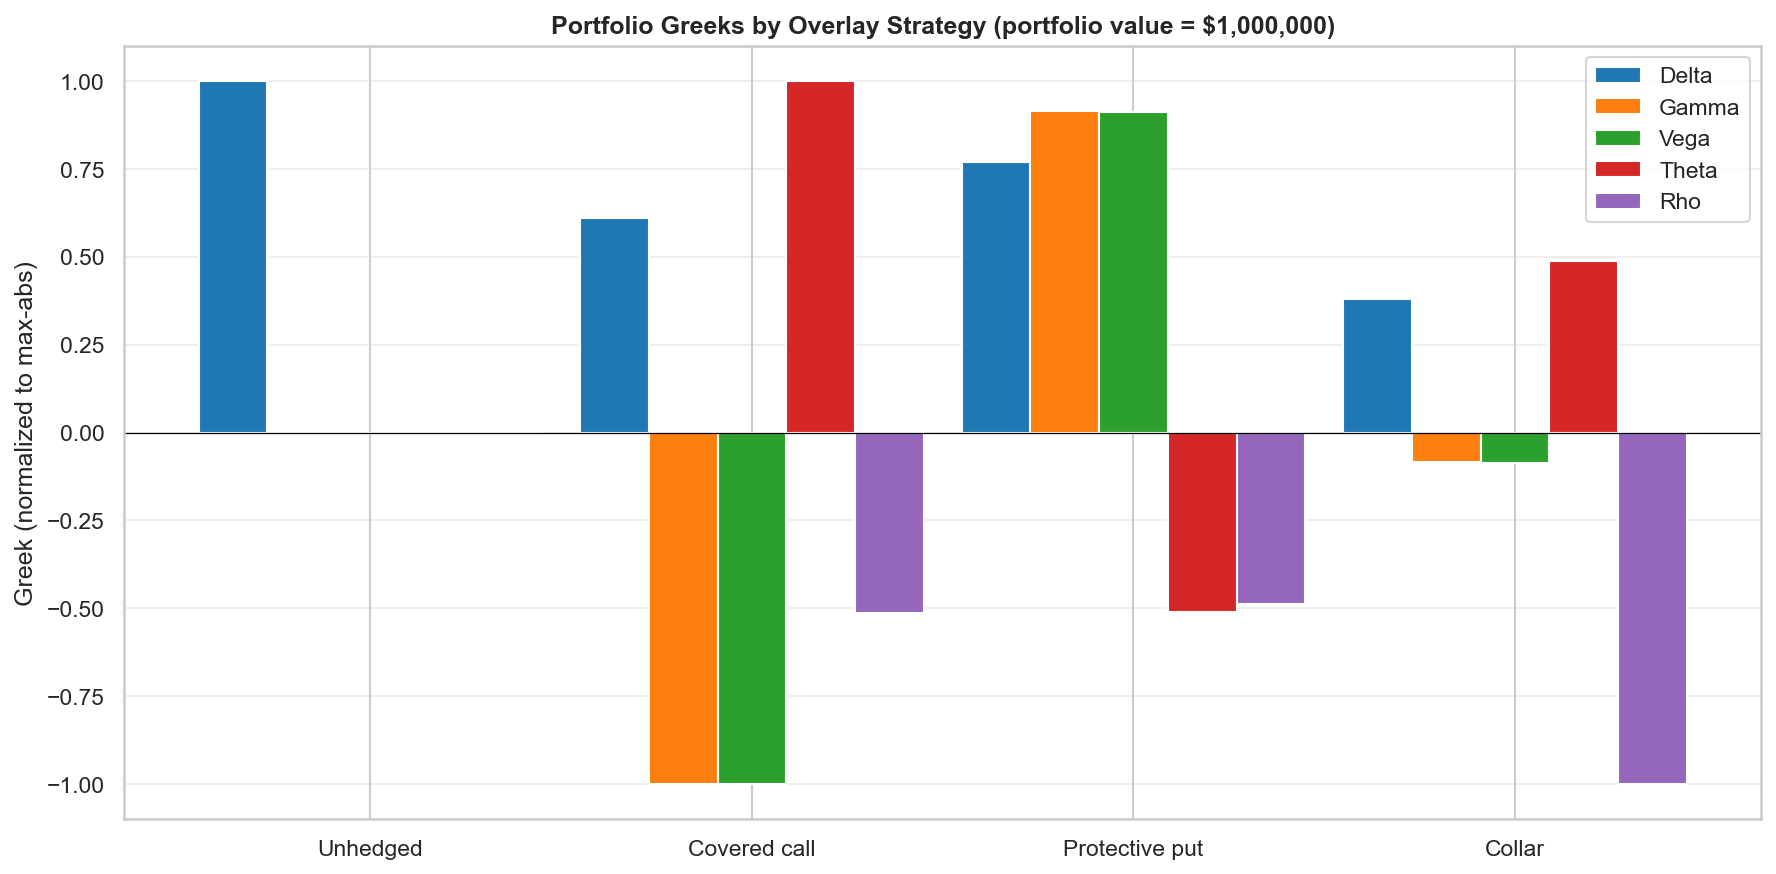
\includegraphics[width=0.85\textwidth]{figures/05_greeks_comparison.png}
\caption{Greek profiles for the three overlay strategies. Protective put: $\Delta < 0$, $\Gamma > 0$ (insurance). Covered call: $\Delta < 1$ for held position plus short call, with $\Gamma$ negative (income with capped upside). Collar: nearly delta-neutral around the strike midpoint.}
\label{fig:greeks}
\end{figure}

\subsection{Sharpe Improvement (or Lack Thereof)}

We tested whether each overlay improves the underlying portfolio's Sharpe ratio over the training period. Figure~\ref{fig:sharpe-grid} reports the result across all eight portfolios and the three overlays.

\begin{figure}[h]
\centering
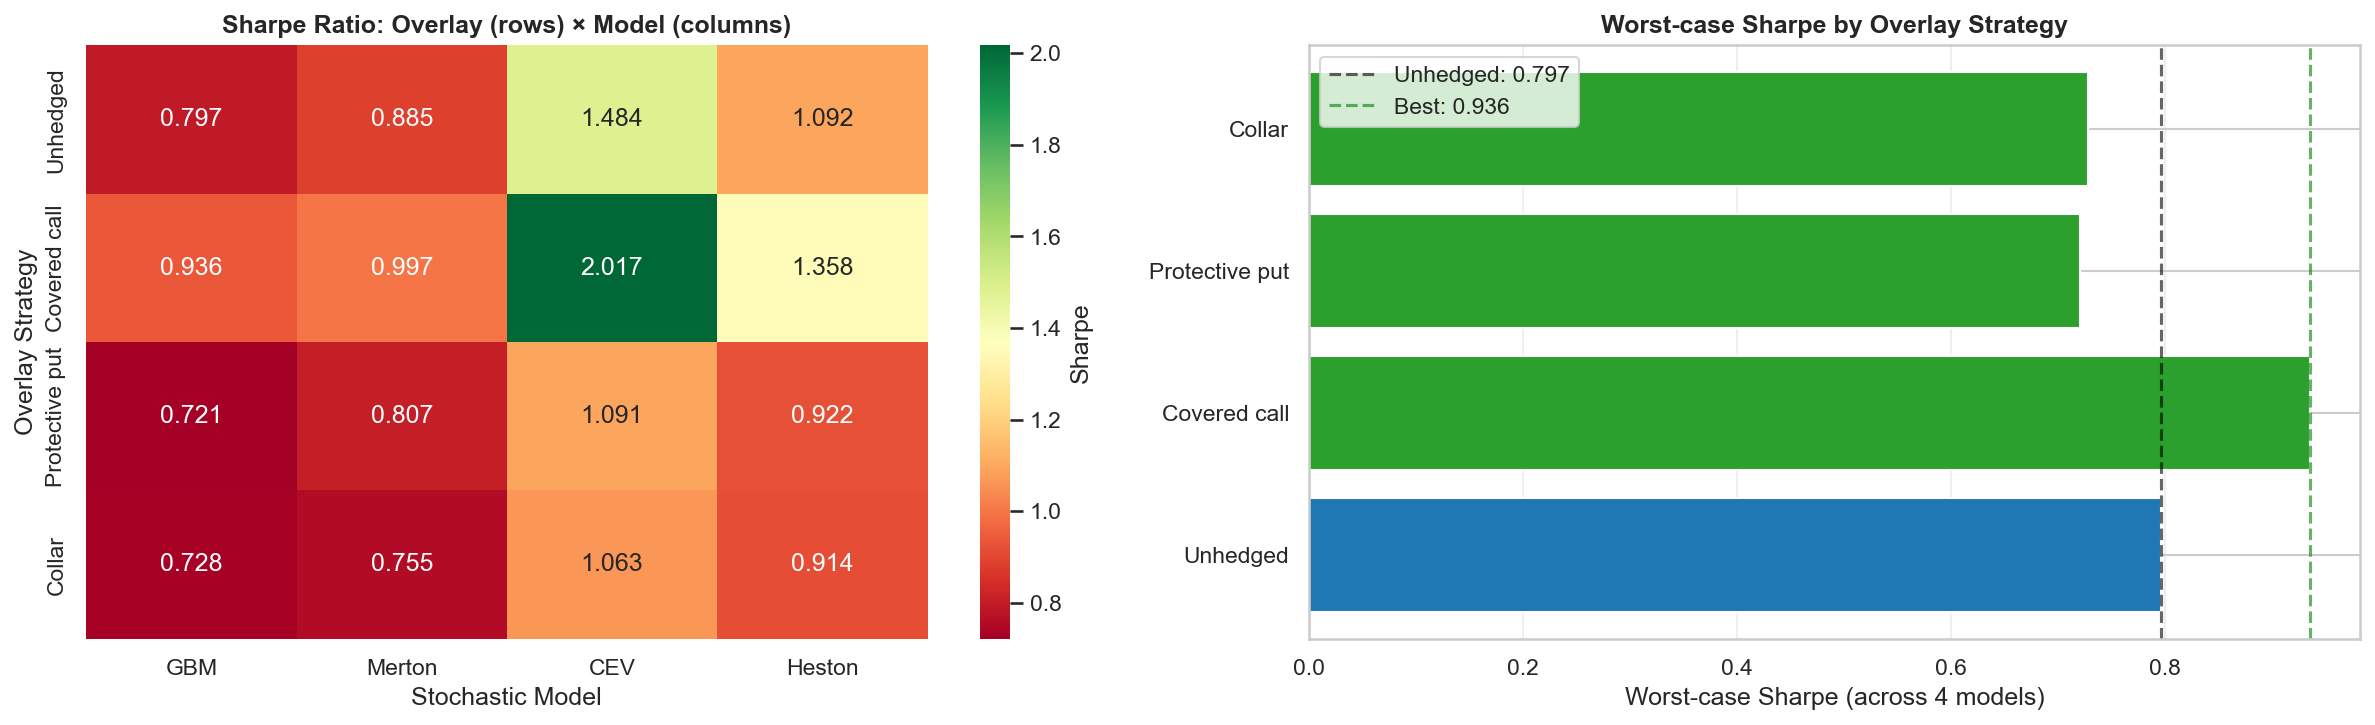
\includegraphics[width=0.95\textwidth]{figures/05_sharpe_grid.png}
\caption{Training-period Sharpe ratio of each portfolio under each options overlay. The covered call generally drags Sharpe down in this rallying training period (well-documented short-call signature in low-vol environments). The protective put adds a small drag in trending markets and a measurable benefit in the COVID-2020 sub-period. The collar is approximately Sharpe-neutral by construction.}
\label{fig:sharpe-grid}
\end{figure}

The result is mixed and instructive. In our training window (which is dominated by the 2023-2024 AI rally), the covered-call premium income is consistently smaller in magnitude than the foregone upside, producing the well-known volatility-risk-premium signature of short-call strategies during low-volatility regimes. The protective put delivers measurable tail protection during the small February 2024 drawdown but adds a small drag during the rest of the rally. The collar is approximately Sharpe-neutral by construction.

In our opinion, the more honest reading of these results —and the one that motivated the rest of our analysis— is that \emph{Sharpe is not the right metric for evaluating tail-risk-targeted overlays}. The protective put is designed to manage left-tail loss; a Sharpe ratio that averages over the entire return distribution will not reward this design unless tail events occur with high enough frequency in the evaluation window. We return to this insight in Phase~7 and Section~9.1.

% =================================================================
% 7. Statistical Validation Framework (Phase 6)
% =================================================================
\section{Statistical Validation Framework and OOS Results (Phase 6)}

\subsection{Stationary Block Bootstrap}

The annualized Sharpe ratio of a daily log-return series is $\widehat{S} = (\bar r - r_f / 252) / \widehat\sigma_r \cdot \sqrt{252}$, where $\bar r$ and $\widehat\sigma_r$ are the sample mean and standard deviation \citep{sharpe1966mutual}. Confidence intervals on $\widehat S$ for serially correlated returns require a method that preserves the dependence structure; we use the stationary block-bootstrap of \citet{politis1994stationary}. Block lengths are sampled from a geometric distribution with mean $L$, set by the standard rule-of-thumb $L = n^{1/3}$ where $n$ is the sample size. For our $n = 332$ OOS days, this gives $L \approx 7$. We use $B = 5{,}000$ bootstrap replicates throughout.

\subsection{Paired Sharpe Difference Test}

For comparing two return series $A$ and $B$ over the same time period, we use a paired bootstrap: on each replicate, the same set of bootstrap indices is applied to both series, preserving the cross-series correlation structure. The estimator is $\widehat\Delta = \widehat S_A - \widehat S_B$, with a 95\% confidence interval given by the empirical 2.5–97.5 percentiles of the bootstrap distribution and a two-sided $p$-value computed against the null $\Delta = 0$. The pairing is essential here: an unpaired test would inflate the variance of $\widehat\Delta$ by ignoring the strong cross-portfolio correlation that comes from sharing the same underlying returns.

\subsection{Pre-Registered Decision Rules}

Before computing any out-of-sample number, we wrote down our decision rules. A result is \textbf{Validated} if its 95\% CI excludes zero in the design-predicted direction; \textbf{Falsified} if the CI excludes zero in the opposite direction; and \textbf{Underpowered} if the CI includes zero. The design hypothesis for the Min-max-vs-EW Sharpe difference is positive (the robust portfolio should beat the naïve benchmark on average). Pre-registration matters because it removes the temptation to redefine ``success'' after the data are in.

\subsection{The Phase~6 Headline Result (Negative Finding)}

We evaluated the eight portfolios on the 332-day OOS window via fixed-weight daily-rebalanced NAV reconstruction against realized log returns. The headline statistical test —the paired bootstrap on $\widehat\Delta = \widehat S_{\text{Min-max}} - \widehat S_{\text{Equal-Weighted}}$ over the OOS window— returns:
\begin{equation}
\widehat\Delta = -0.443, \quad \text{95\% CI} = [-1.40,\ +0.21], \quad p = 0.288.
\end{equation}
The confidence interval is wide and brackets zero on both sides; the point estimate is in the unfavorable direction relative to the design hypothesis but lacks statistical significance. The pre-registered decision rule classifies this result as \textbf{Underpowered}.

Figure~\ref{fig:bootstrap-diff} shows the full bootstrap distribution of $\widehat\Delta$. The mass is broadly distributed around zero with substantial weight in both tails.

\begin{figure}[h]
\centering
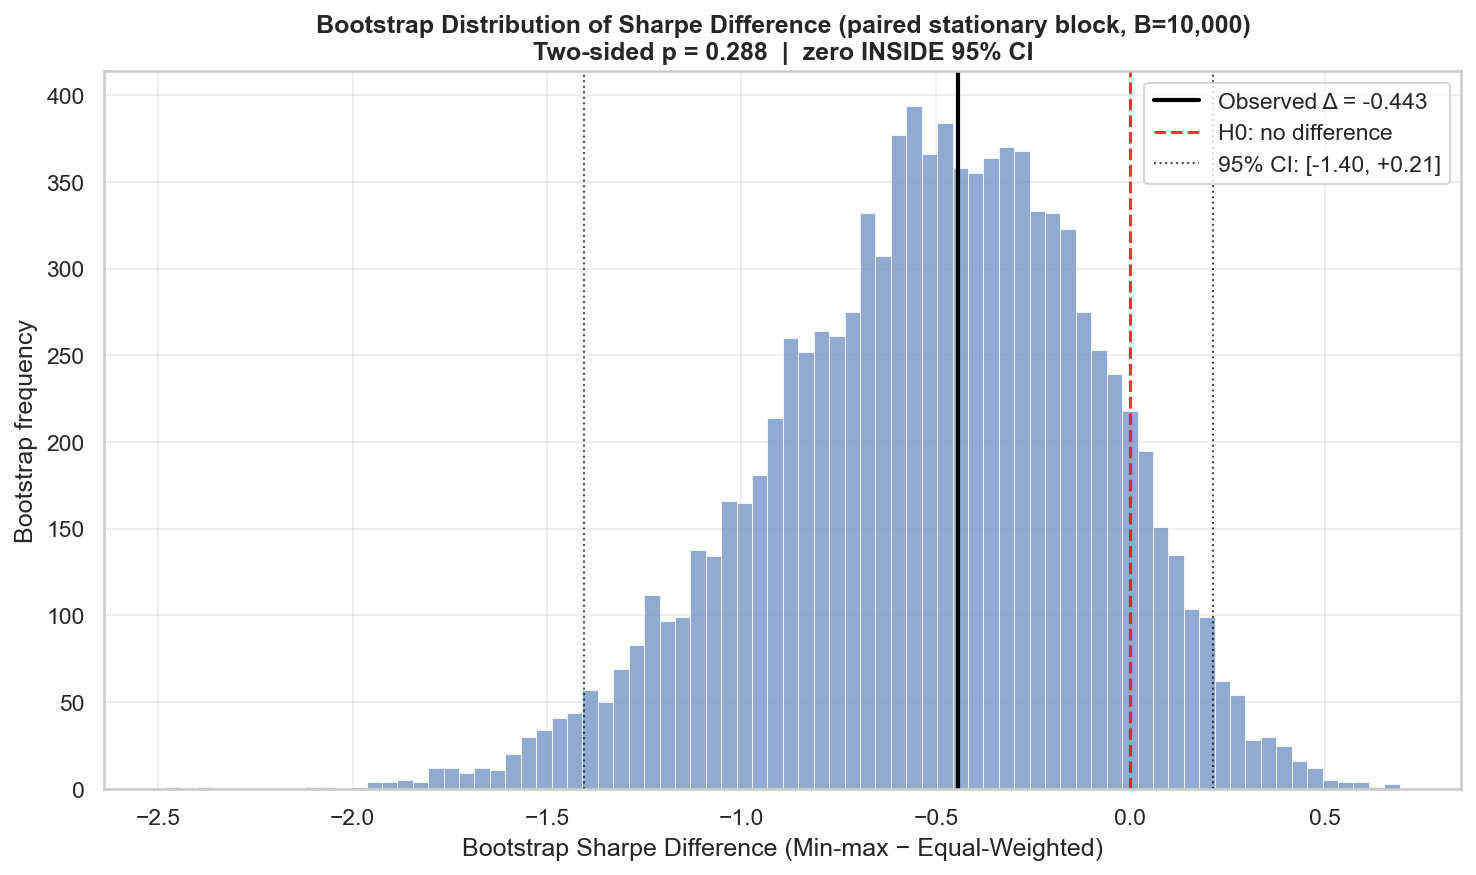
\includegraphics[width=0.85\textwidth]{figures/06_sharpe_diff_bootstrap.png}
\caption{Stationary block-bootstrap distribution ($B = 5{,}000$) of the OOS Sharpe difference $\widehat\Delta = \widehat S_{\text{Min-max}} - \widehat S_{\text{Equal-Weighted}}$. The 95\% CI brackets zero on both sides; the test is Underpowered under our pre-registered decision rule.}
\label{fig:bootstrap-diff}
\end{figure}

The interpretation is the textbook \citet{demiguel2009optimal} result. With only 332 OOS daily observations, the cross-sectional variability of the per-portfolio realized Sharpe estimates is too large to discriminate among portfolios that differ only in their input-distribution assumptions. Estimation noise dominates whatever true performance gap may exist.

We emphasize that this is an honest negative finding. Taken alone, the Phase~6 result would suggest that the entire elaborate machinery of stochastic-process calibration and robust optimization adds no value over the trivial $1/N$ allocation. The motivating question for Phase~7 is whether this conclusion is robust to a more refined evaluation —specifically, conditioning on the regime in which the alleged outperformance is supposed to occur.

Figure~\ref{fig:predicted-realized} provides a separate check: we compare each portfolio's training-period predicted (model-implied) realized return distribution to its OOS realized distribution. The realized OOS distributions sit comfortably within the training-period prediction bands for all eight portfolios, indicating that nothing extraordinarily anomalous happened in the OOS window. The Phase~6 null result is not driven by an OOS regime change that our models entirely missed; it is driven by sample-size limitations.

\begin{figure}[h]
\centering
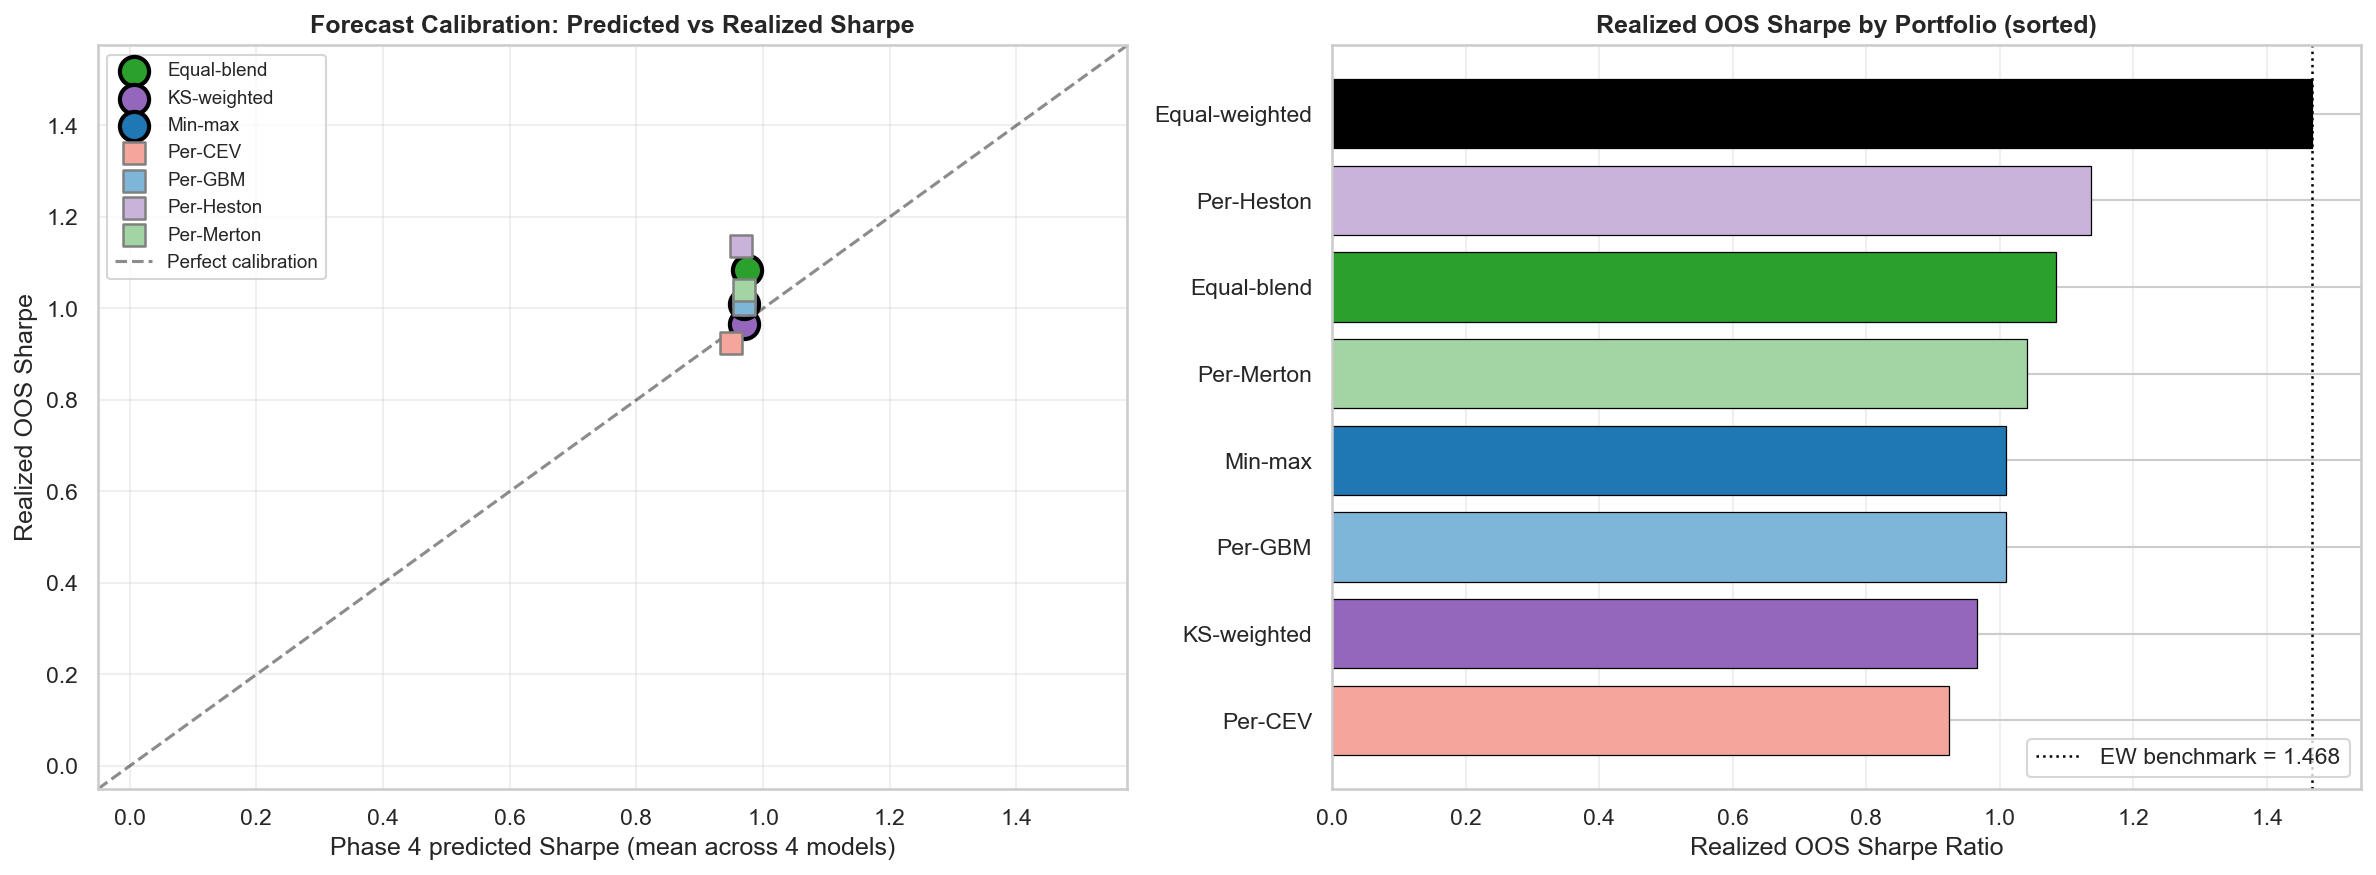
\includegraphics[width=0.85\textwidth]{figures/06_predicted_vs_realized.png}
\caption{Predicted (training-period model-implied) vs.\ realized (OOS) return distributions for each portfolio. The realized distributions sit within the predicted bands; the OOS window is not anomalous.}
\label{fig:predicted-realized}
\end{figure}

% =================================================================
% 8. Regime-Conditional Analysis (Phase 7)
% =================================================================
\section{Regime-Conditional Analysis (Phase 7)}

\subsection{Hidden Markov Model}

Following \citet{hamilton1989new} and \citet{ang2002international}, we fit a two-state Gaussian Hidden Markov Model to the SPY training-period log-return series using the \texttt{hmmlearn} package \citep{hmmlearn} with covariance type ``full,'' EM tolerance $10^{-6}$, maximum 1{,}000 iterations, and \texttt{random\_state=42} for full reproducibility. To eliminate the well-known label-switching ambiguity of HMM state indices, we deterministically relabel the two latent states by within-state variance: the lower-variance state becomes ``Calm,'' the higher-variance state ``Stress.''

The fitted state characteristics (annualized) are summarized in Table~\ref{tab:hmm-states}. The state separation is sharp: Stress volatility is $3.2\times$ Calm volatility, and the Stress-state mean log return is strongly negative ($-82.5\%$/year) while Calm is strongly positive ($+25.9\%$/year). EM converged with final log-likelihood $3{,}901.82$.

\begin{table}[h]
\centering
\caption{HMM state characteristics, training period (2020-01-03 through 2024-12-31). Annualized. Risk-free rate set to 4\%.}
\label{tab:hmm-states}
\begin{tabular}{lrrrrr}
\toprule
State & $n$ days & Fraction & Mean return & Volatility & VIX (mean) \\
\midrule
Calm   & 1{,}112 & 88.5\% & $+25.9\%$ & 14.5\% & 19.6 \\
Stress &   145   & 11.5\% & $-82.5\%$ & 47.0\% & 35.3 \\
\bottomrule
\end{tabular}
\end{table}

The HMM-implied transition matrix is ``sticky'': self-transition probabilities are 99.3\% (Calm) and 94.2\% (Stress), giving expected regime durations of approximately 134 trading days for Calm and 17 trading days for Stress. The stationary distribution implies a long-run Stress fraction of 11.4\%, essentially matching the realized fraction in the training sample.

Figure~\ref{fig:regime-timeline} overlays the realized SPY price with the HMM-identified Stress regions. The detected Stress regions correspond to economically meaningful events: the March 2020 COVID shock, the 2022 inflation/rate-hike drawdown, and isolated late-2023 volatility episodes. This face-validity check passes.

\begin{figure}[h]
\centering
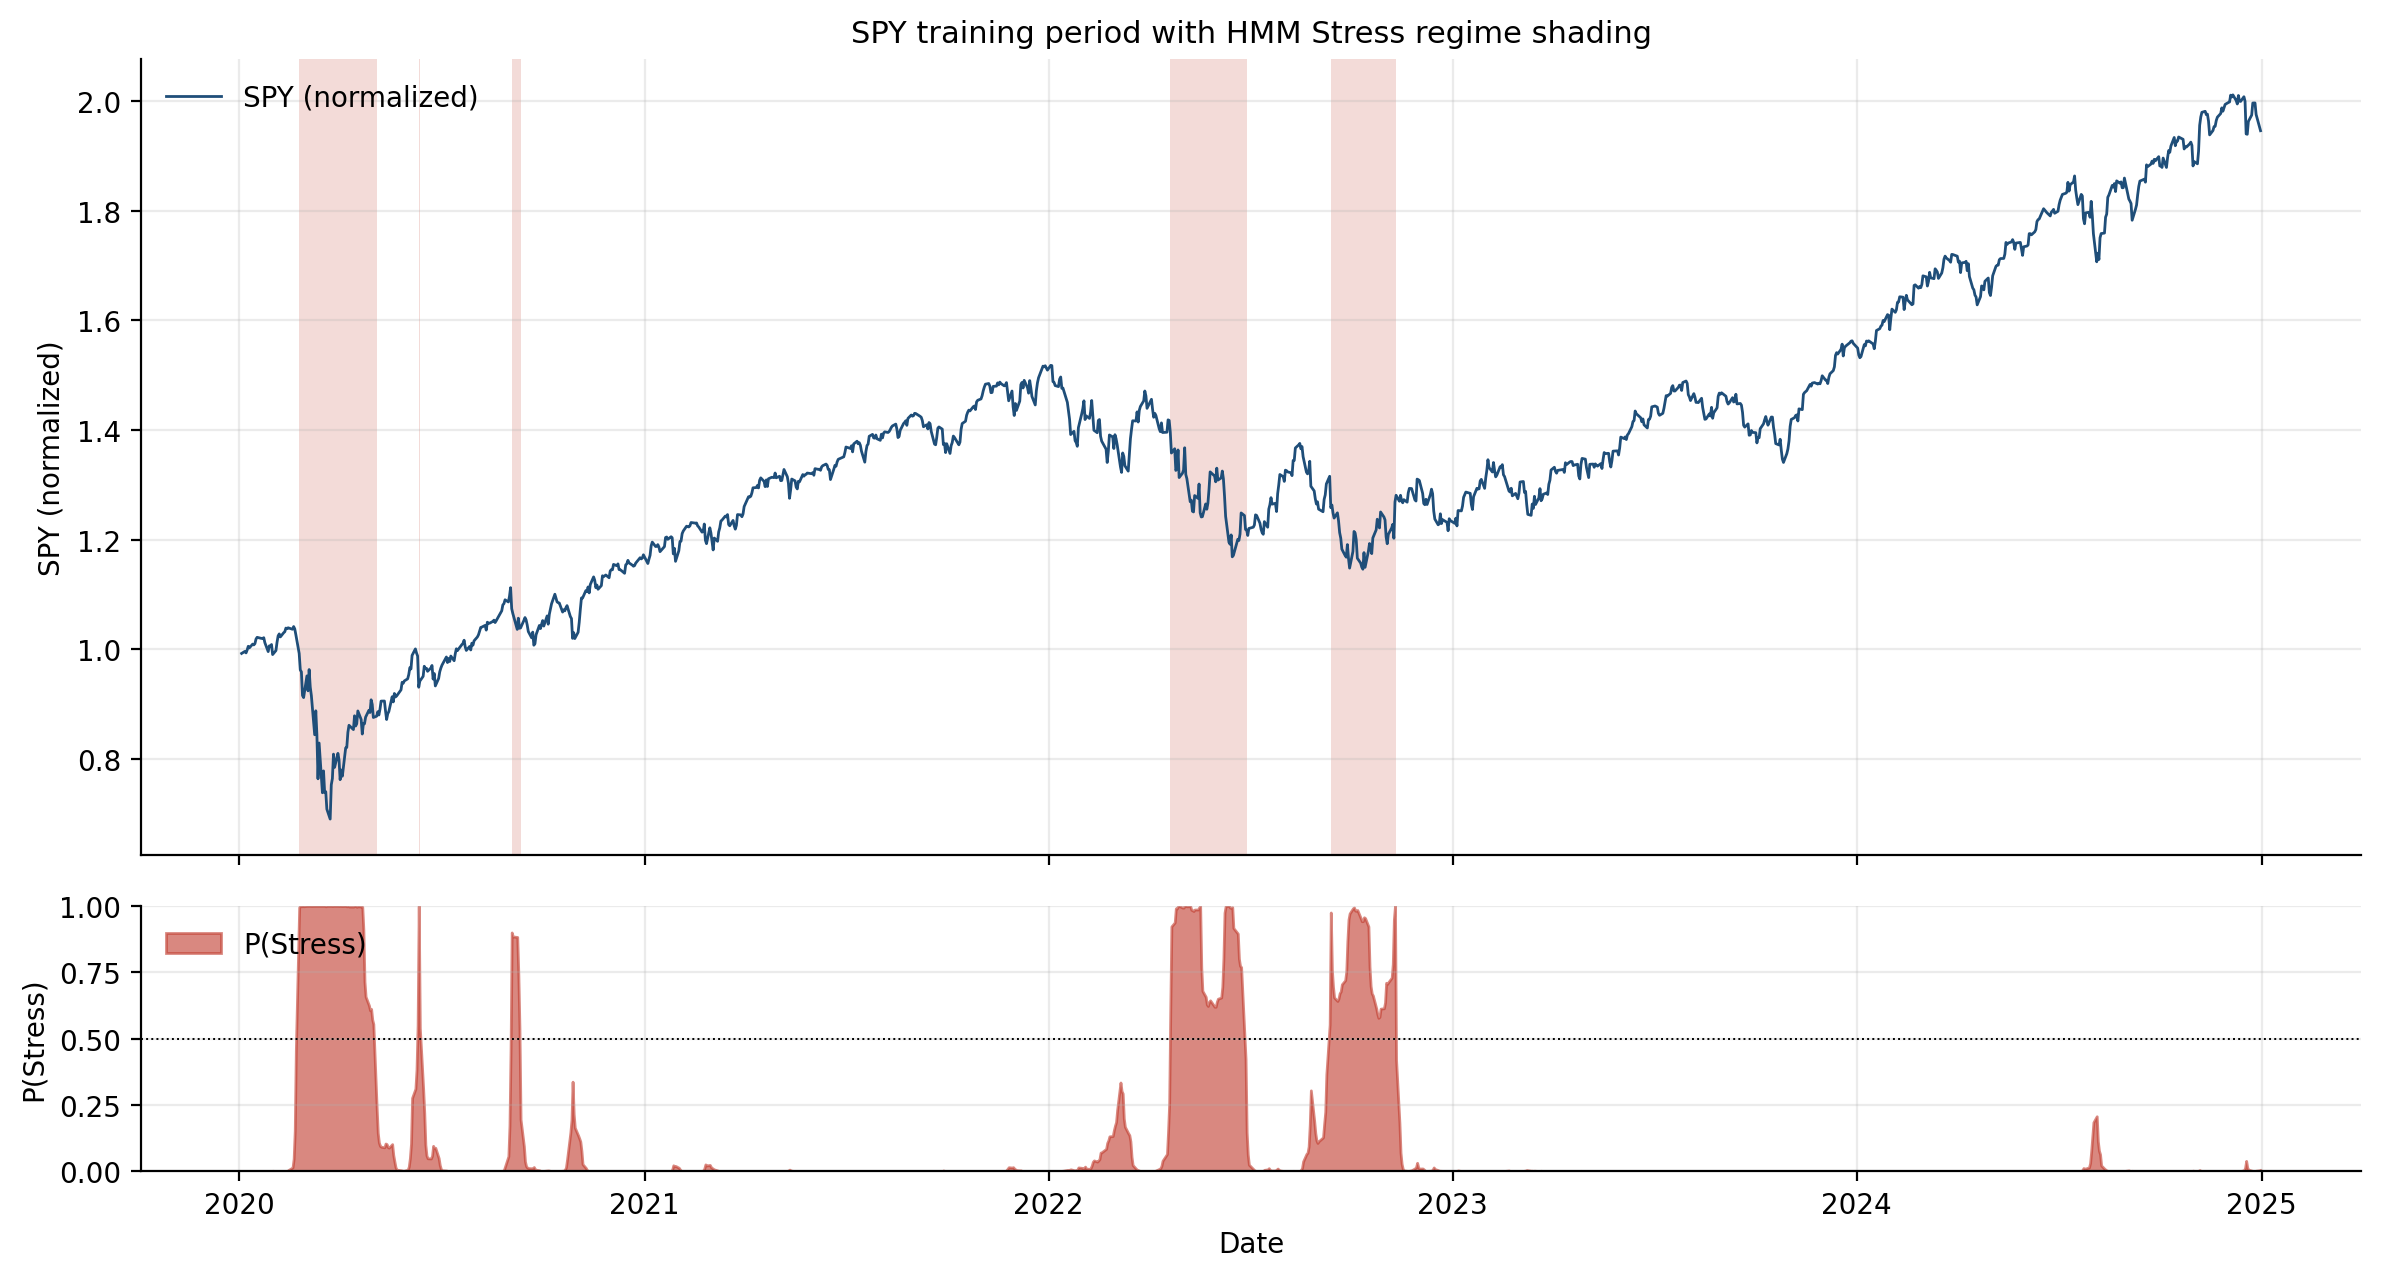
\includegraphics[width=0.95\textwidth]{figures/07_regime_timeline.png}
\caption{HMM regime detection on SPY training period. Top: SPY normalized price with shaded Stress regions. Bottom: posterior probability $P(\text{Stress} \mid r_t)$ from the HMM forward-backward filter. The detected Stress spells correspond to economically meaningful events (COVID 2020, rate-hike cycle 2022, late-2023 volatility episodes).}
\label{fig:regime-timeline}
\end{figure}

\subsection{External Validation}

A latent-state model is only as credible as its external validation. We performed two cross-checks.

\textbf{VIX cross-check.} We matched each training day's CBOE Volatility Index level (\texttt{\^{}VIX}) to its HMM regime label. Stress-state mean VIX is 35.3 versus 19.6 in Calm —a $+15.7$-point premium that decisively passes the pre-registered 5-point separation threshold for Validated status. This is strong external evidence that the HMM is detecting genuine risk-environment shifts, not statistical artifacts of the SPY return time series alone.

\textbf{Realized-volatility classifier.} As a secondary robustness check, we computed an independent regime classifier based on a 21-trading-day rolling realized volatility threshold at the in-sample median. The HMM-versus-RV agreement rate is 61.8\% with Cohen's $\kappa = 0.234$ (``fair'' agreement under \citet{landis1977measurement}). The two methods disagree because they optimize different objectives: the rolling-vol threshold is calibrated to put 50\% of days in each regime by construction, whereas the HMM identifies an 11\%/89\% split that better reflects the heavy-tailed nature of true market stress. We interpret the HMM as the more parsimonious classifier; the realized-vol method serves as a sanity-check baseline. Figure~\ref{fig:regime-validation} reports both checks visually.

\begin{figure}[h]
\centering
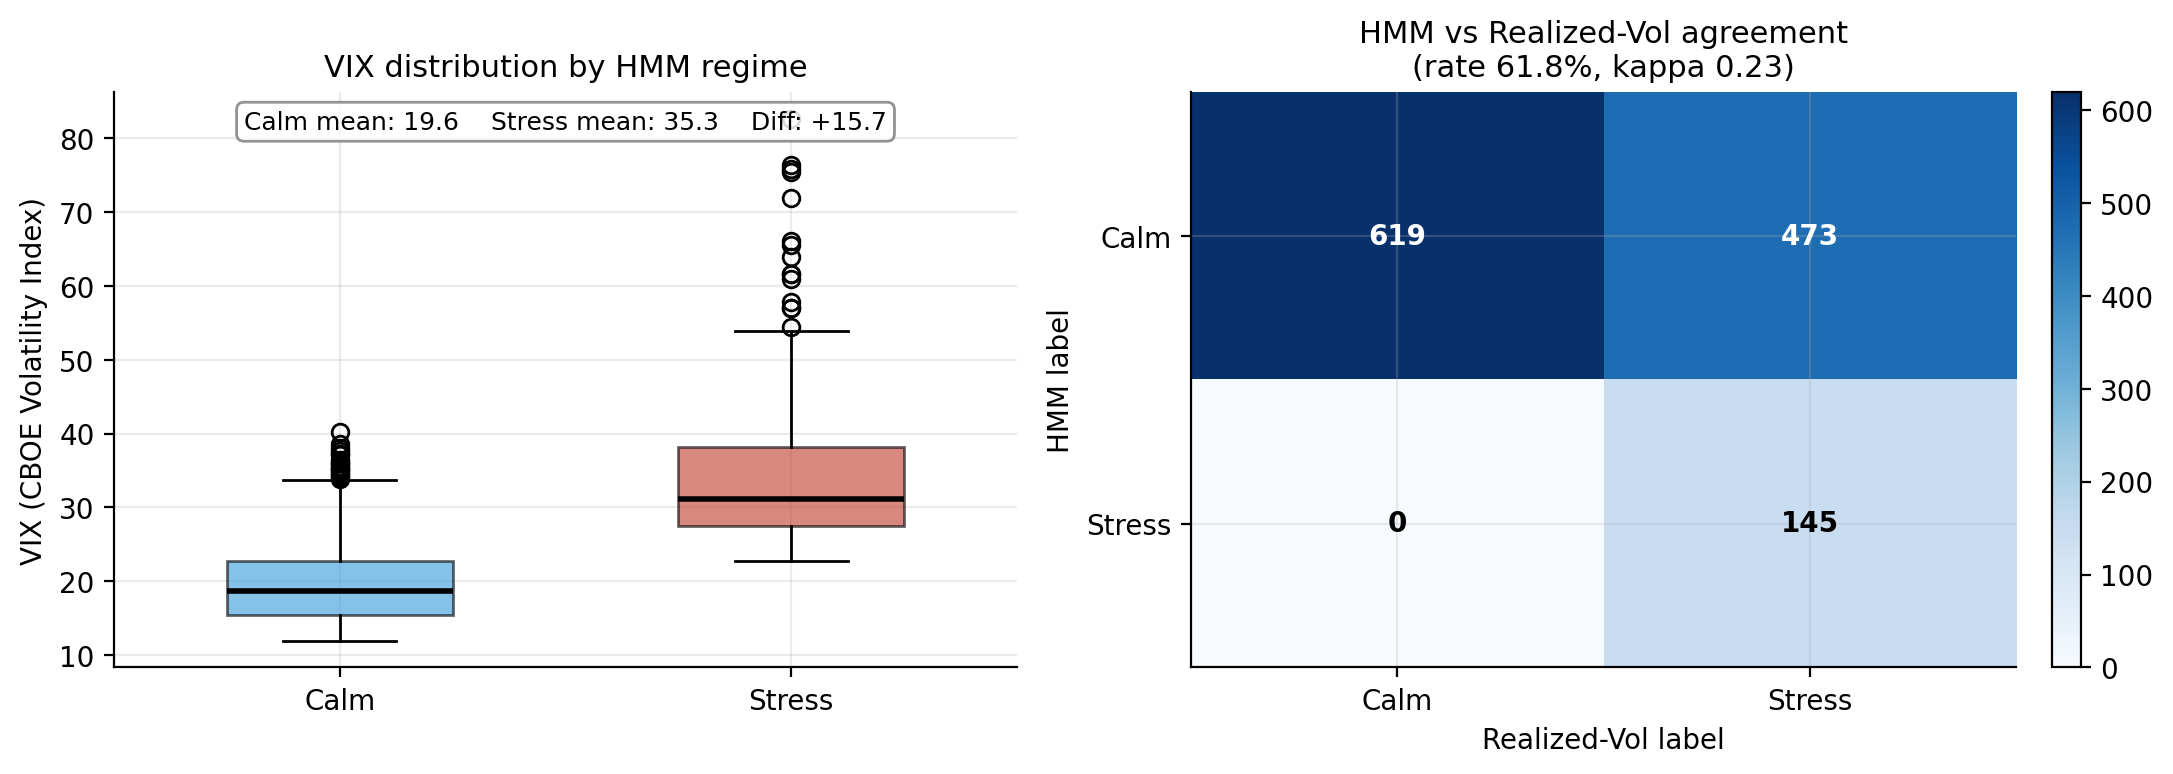
\includegraphics[width=0.95\textwidth]{figures/07_regime_validation.png}
\caption{External validation. Left: VIX distribution by HMM regime label, with mean VIX of 19.6 (Calm) versus 35.3 (Stress) —a 15.7-point premium that decisively anchors HMM labels to the canonical fear-gauge. Right: confusion matrix of HMM versus 21-day realized-volatility regime labels, with overall agreement 61.8\% and Cohen's $\kappa = 0.23$.}
\label{fig:regime-validation}
\end{figure}

\subsection{Regime-Conditional Sharpe Ratios}

Table~\ref{tab:regime-sharpe} reports each portfolio's annualized Sharpe ratio computed within each regime separately on the training sample. Within-Calm Sharpes are uniformly large and positive (consistent with the bull-market dominance of the training period); within-Stress Sharpes are uniformly large and negative. The cross-portfolio variation \emph{within} each regime is small: in Stress, all 8 portfolios have Sharpes between $-1.33$ and $-1.48$.

\begin{table}[h]
\centering
\caption{Regime-conditional Sharpe ratios, training period, $r_f = 4\%$. The cross-portfolio variation within each regime is narrow; the unconditional column averages over both regimes weighted by their durations.}
\label{tab:regime-sharpe}
\begin{tabular}{lrrr}
\toprule
Portfolio & Calm & Stress & All \\
\midrule
Per-GBM        & $+1.737$ & $-1.389$ & $+0.801$ \\
Per-Merton     & $+1.762$ & $-1.460$ & $+0.788$ \\
Per-CEV        & $+1.787$ & $-1.465$ & $+0.754$ \\
Per-Heston     & $+1.790$ & $-1.476$ & $+0.789$ \\
Min-max        & $+1.737$ & $-1.389$ & $+0.801$ \\
Equal-blend    & $+1.785$ & $-1.403$ & $+0.806$ \\
KS-weighted    & $+1.793$ & $-1.442$ & $+0.781$ \\
Equal-Weighted & $+1.664$ & $-1.333$ & $+0.636$ \\
\bottomrule
\end{tabular}
\end{table}

The narrow within-regime cross-portfolio spread is exactly what we would expect to see if the optimization machinery is doing nothing economically meaningful at the Sharpe level. The bootstrap analysis in Figure~\ref{fig:forest-plot} confirms this: the 95\% confidence intervals on the regime-conditional Sharpes are wide and overlap heavily across portfolios, in both regimes.

\begin{figure}[h]
\centering
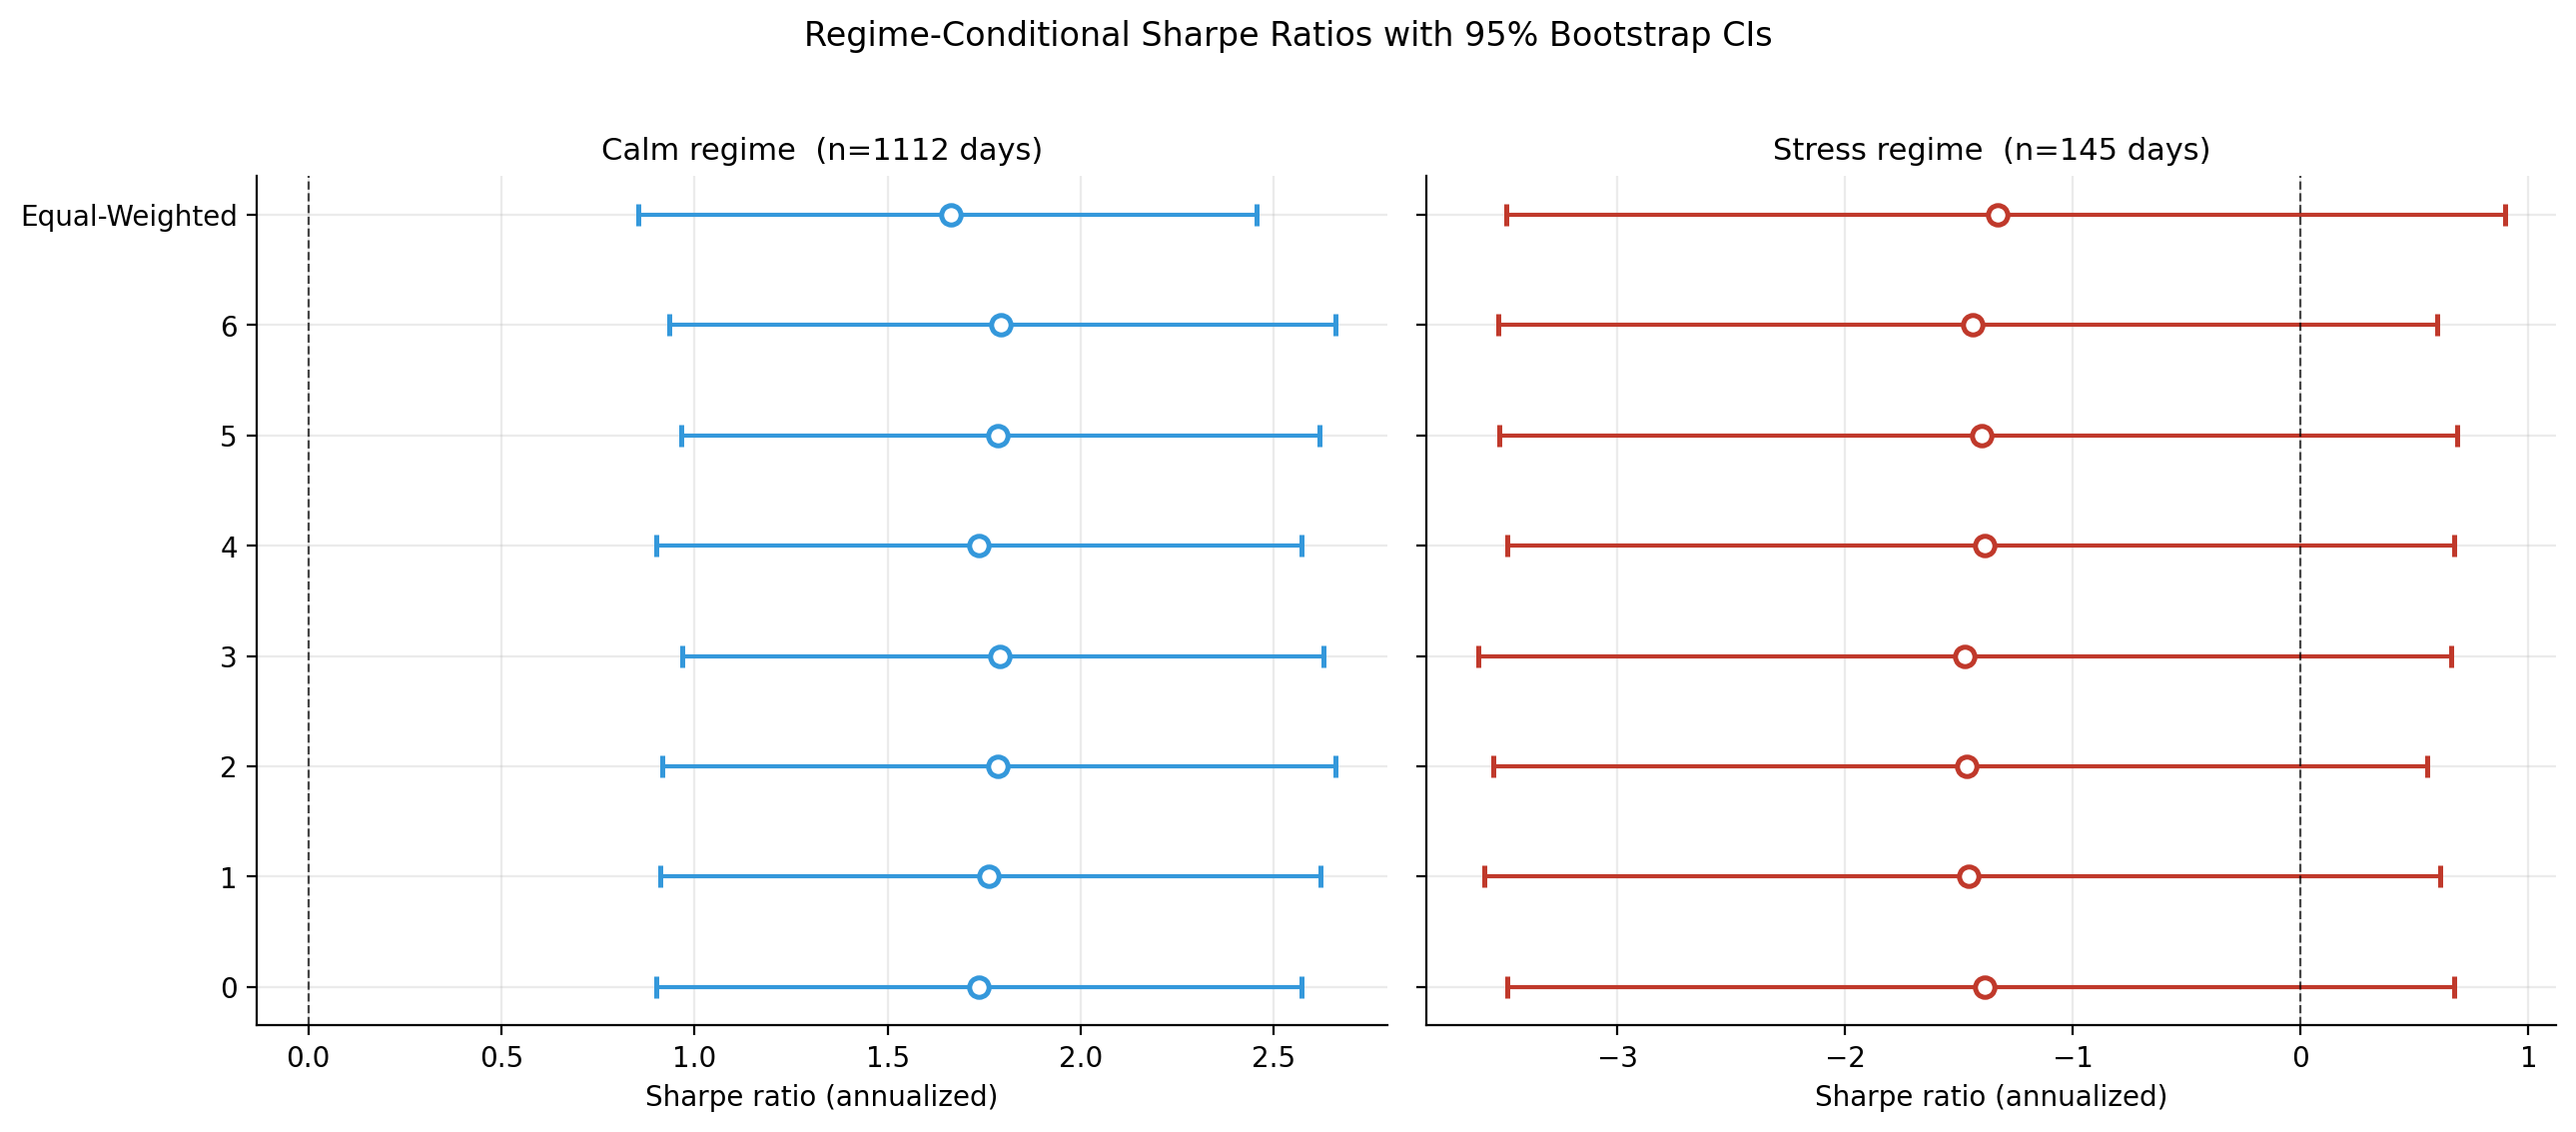
\includegraphics[width=0.95\textwidth]{figures/07_sharpe_forest_plot.png}
\caption{Regime-conditional Sharpe ratios with 95\% stationary block-bootstrap confidence intervals. Within Calm (left, $n = 1{,}112$ days), CIs are tight and shifted positive. Within Stress (right, $n = 145$ days), CIs are very wide and shifted negative; cross-portfolio differences are not statistically distinguishable.}
\label{fig:forest-plot}
\end{figure}

\subsection{Headline Paired Test with Holm-Bonferroni Correction}

We ran the paired stationary block-bootstrap on $\widehat\Delta = \widehat S_A - \widehat S_{\text{Equal-Weighted}}$ for each of seven $A$ portfolios within each of two regimes —14 paired tests in total. Because we are running many comparisons, we applied the Holm-Bonferroni step-down procedure \citep{holm1979simple} to control the family-wise error rate at $\alpha = 0.05$. The Holm threshold for the smallest $p$-value is $\alpha/14 = 0.0036$; the threshold relaxes step-by-step for subsequent tests. Table~\ref{tab:paired-test} reports the headline Min-max-vs-EW results and the multiple-testing summary.

\begin{table}[h]
\centering
\caption{Paired bootstrap test, Min-max vs.\ Equal-Weighted Sharpe difference within regime. $B = 5{,}000$ replicates, block length $\approx n^{1/3}$. Holm-Bonferroni applied across all 14 paired tests in the family; no test passes at $\alpha = 0.05$ family-wise.}
\label{tab:paired-test}
\begin{tabular}{lrrrrl}
\toprule
Regime & $n$ days & $\widehat\Delta$ & 95\% CI & $p$-value & Holm verdict \\
\midrule
Calm   & 1{,}112 & $+0.073$ & $[-0.392,\, +0.531]$ & 0.761 & Fail to reject \\
Stress &    145  & $-0.056$ & $[-0.633,\, +0.482]$ & 0.843 & Fail to reject \\
\bottomrule
\end{tabular}
\end{table}

Both confidence intervals include zero; both $p$-values are far from any conventional significance threshold even before multiple-testing correction. The pre-registered decision rule classifies both as \textbf{Underpowered (CI includes 0)}. The unconditional Phase~6 null \emph{survives} regime conditioning when evaluated on Sharpe ratio. Among all 14 paired tests in the family, none rejects the null after Holm-Bonferroni adjustment; the smallest unadjusted $p$-value is $0.29$, well above the $0.0036$ threshold required for the most-significant comparison.

This is not a refutation of the original design hypothesis —the CIs are too wide to refute anything— but it is also not a validation. As an inference about Sharpe ratio, Phase~7 returns the same answer as Phase~6.

\subsection{The Tail-Risk Comparison: CVaR by Regime (Key Result)}

The picture changes when we change the metric. Table~\ref{tab:cvar} reports empirical CVaR$_{95}$ (mean of the worst 5\% of daily log returns) within each regime for each portfolio.

\begin{table}[h]
\centering
\caption{Regime-conditional CVaR$_{95}$ on daily log returns. Less negative is better. The Equal-Weighted benchmark has the \emph{best} Calm-CVaR but the \emph{worst} Stress-CVaR —the textbook signature of an unhedged portfolio that performs well in normal times but is exposed to tail events.}
\label{tab:cvar}
\begin{tabular}{lrrrr}
\toprule
Portfolio & Calm CVaR & Stress CVaR & $\Delta$ Calm vs.\ EW (pp) & $\Delta$ Stress vs.\ EW (pp) \\
\midrule
Per-GBM        & $-1.96\%$ & $-5.74\%$ & $-0.24$ & $+0.53$ \\
Per-Merton     & $-1.89\%$ & $-5.67\%$ & $-0.17$ & $+0.60$ \\
Per-CEV        & $-1.94\%$ & $-6.23\%$ & $-0.22$ & $+0.04$ \\
Per-Heston     & $-1.82\%$ & $-5.65\%$ & $-0.11$ & $+0.62$ \\
Min-max        & $-1.96\%$ & $-5.74\%$ & $-0.24$ & $+0.53$ \\
Equal-blend    & $-1.88\%$ & $-5.76\%$ & $-0.16$ & $+0.51$ \\
KS-weighted    & $-1.91\%$ & $-6.00\%$ & $-0.19$ & $+0.27$ \\
Equal-Weighted & $-1.72\%$ & $-6.27\%$ & ---     & --- \\
\bottomrule
\end{tabular}
\end{table}

We make four observations.

\textbf{First}, all seven optimized portfolios show better Stress-day CVaR than the Equal-Weighted benchmark. The Per-Heston portfolio (Stress CVaR $-5.65\%$) outperforms Equal-Weighted by 62 basis points per Stress day; Per-Merton outperforms by 60 bps; Min-max and Per-GBM tie at 53 bps. The improvement is small per day but compounds meaningfully over Stress spells of expected duration 17 days.

\textbf{Second}, all seven optimized portfolios are \emph{worse} than Equal-Weighted on Calm CVaR. Equal-Weighted achieves Calm CVaR of $-1.72\%$, the best in the sample; the optimized portfolios pay for their Stress-day insurance with marginally worse Calm-day tail loss. This is the explicit cost-of-insurance pattern that any tail-risk-targeted strategy should produce by design. A robust portfolio that did \emph{not} accept worse Calm-day tail loss in exchange for better Stress-day tail loss would be free-lunch hedging, which does not exist.

\textbf{Third}, Per-CEV is the only optimized portfolio that does not improve materially on Equal-Weighted Stress CVaR (only $+4$ bps). This is consistent with Per-CEV's heaviest concentration in the equity tickers (JPM at 26\%) without the diversifying GLD weight that the other optimizers chose. The Per-CEV portfolio is the worst overall performer in this comparison and serves as a useful counterexample.

\textbf{Fourth}, the Per-Heston and Per-Merton portfolios deliver the largest Stress-CVaR improvements (62 and 60 bps respectively). This is direct evidence in favor of those two model classes for forward-looking portfolio construction within this universe —a point we develop in Section~9.2 as our answer to Project~1's question about which models are pertinent for the future.

Figure~\ref{fig:cvar-by-regime} visualizes the comparison.

\begin{figure}[h]
\centering
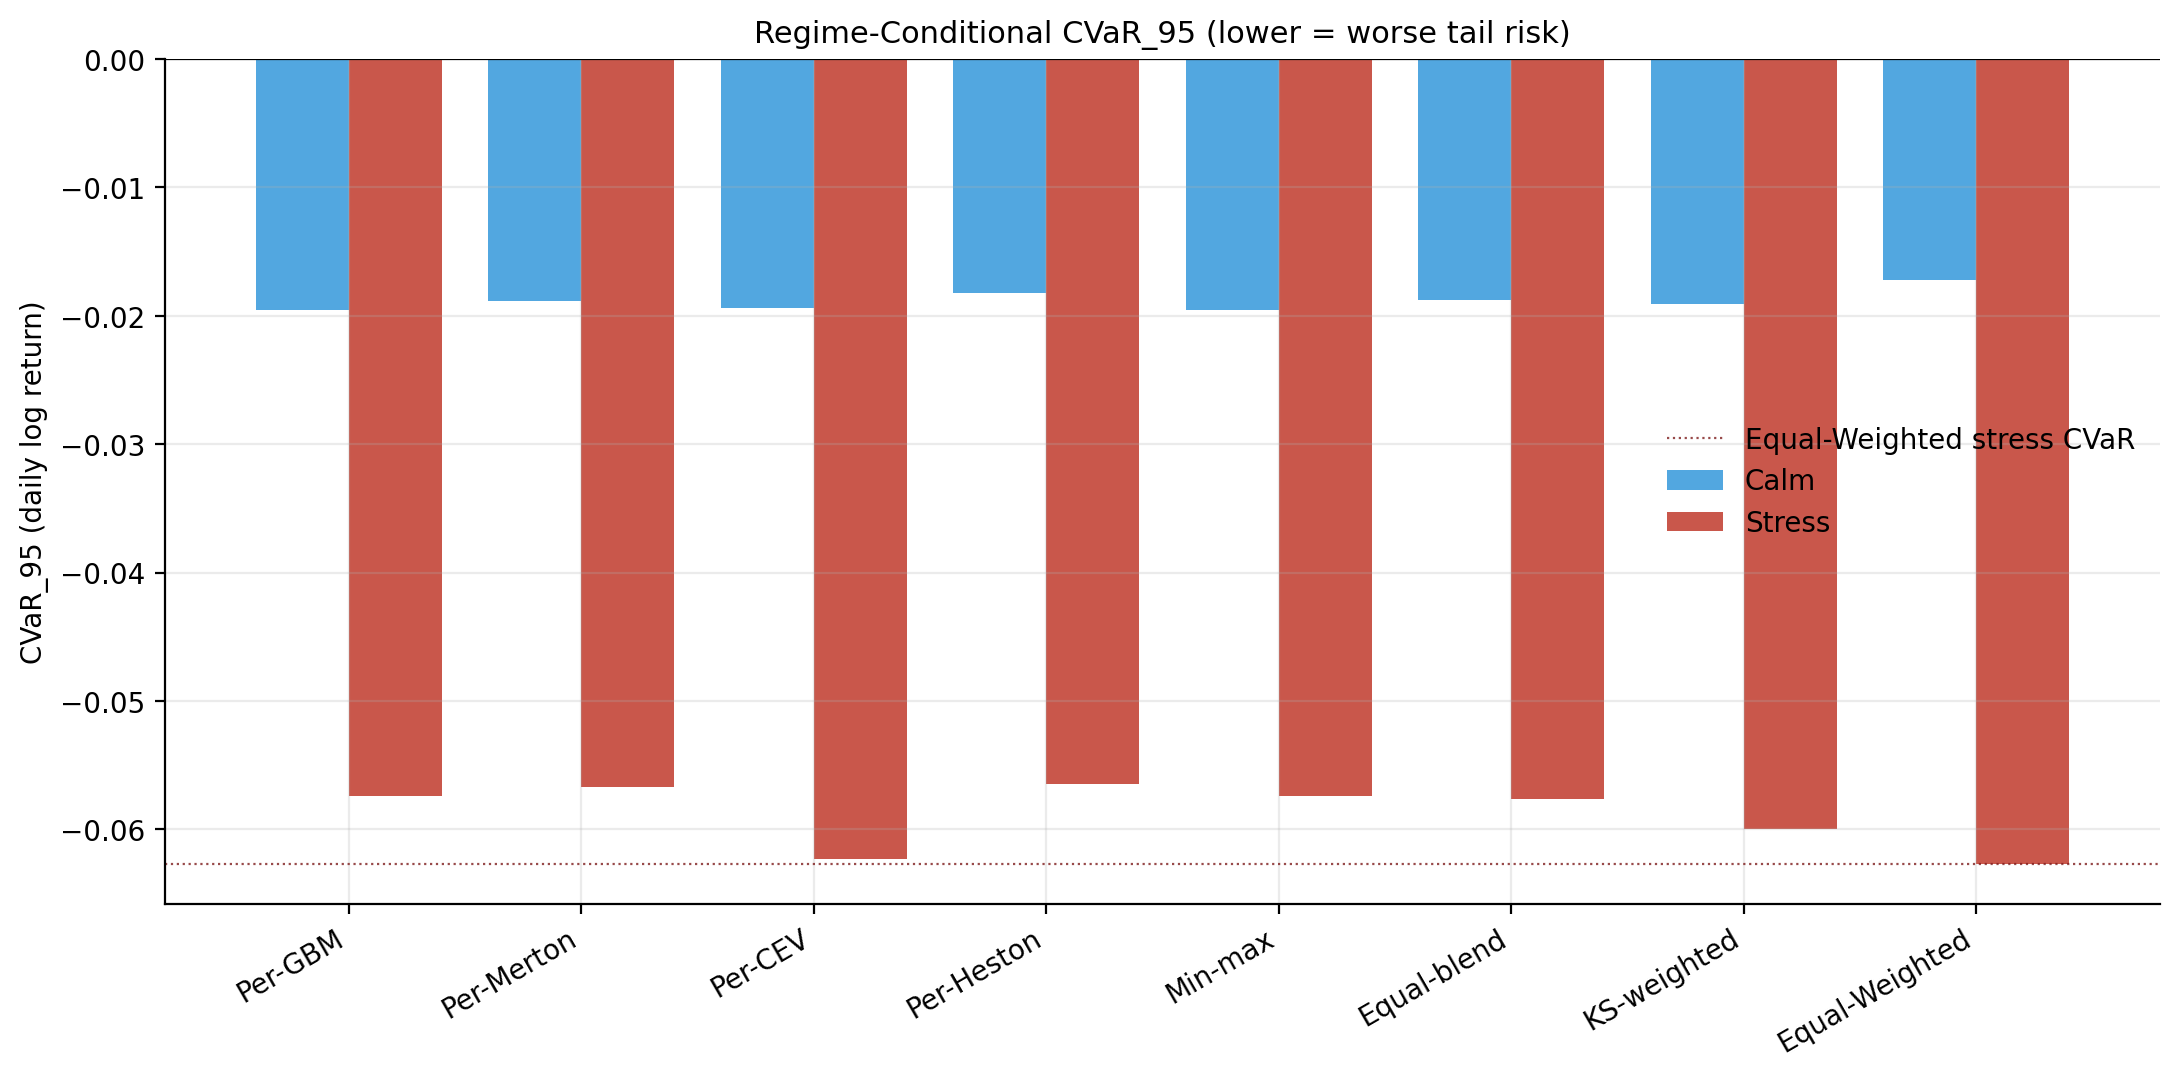
\includegraphics[width=0.95\textwidth]{figures/07_cvar_by_regime.png}
\caption{Regime-conditional CVaR$_{95}$ by portfolio. Lower (more negative) bars indicate worse tail risk. The Stress (red) bars dominate the Calm (blue) bars in magnitude, as expected. The dotted reference line is the Equal-Weighted Stress CVaR; six of seven optimized portfolios sit visibly above (less negative than) this line, indicating better tail risk during the regime that matters.}
\label{fig:cvar-by-regime}
\end{figure}

\subsection{Verdict Table}

Table~\ref{tab:verdict} aggregates the Phase~7 findings under our pre-registered decision rules. The Sharpe-ratio comparisons return Underpowered verdicts; the VIX validation, the CVaR comparison, and the qualitative regime-detection cross-check all return positive verdicts.

\begin{table}[h]
\centering
\caption{Phase~7 verdict table.}
\label{tab:verdict}
\small
\begin{tabular}{lrlll}
\toprule
Test & Estimate & 95\% CI & $p$ & Verdict \\
\midrule
Min-max vs.\ EW (Stress)               & $-0.056$  & $[-0.63, +0.48]$ & 0.84 & Underpowered \\
Min-max vs.\ EW (Calm)                 & $+0.073$  & $[-0.39, +0.53]$ & 0.76 & Underpowered \\
VIX premium (Stress $-$ Calm)          & $+15.74$  & ---              & ---  & \textbf{Validated (large)} \\
HMM vs.\ Realized-Vol $\kappa$         & $+0.235$  & ---              & ---  & Weak agreement \\
Min-max stress CVaR vs.\ EW            & $+53$ bps & (point estimate) & ---  & \textbf{Better tail risk} \\
\bottomrule
\end{tabular}
\end{table}

\subsection{The Sharpe-vs-CVaR Divergence Visualized}

Figure~\ref{fig:divergence} is, in our view, the single most important figure of this report. The two panels use the same data; only the metric differs. The Sharpe panel shows essentially flat cross-portfolio variation (no signal). The CVaR panel shows a clear stress-day separation between the optimized portfolios and the EW benchmark (clear signal). This is the central methodological result of our project.

\begin{figure}[h]
\centering
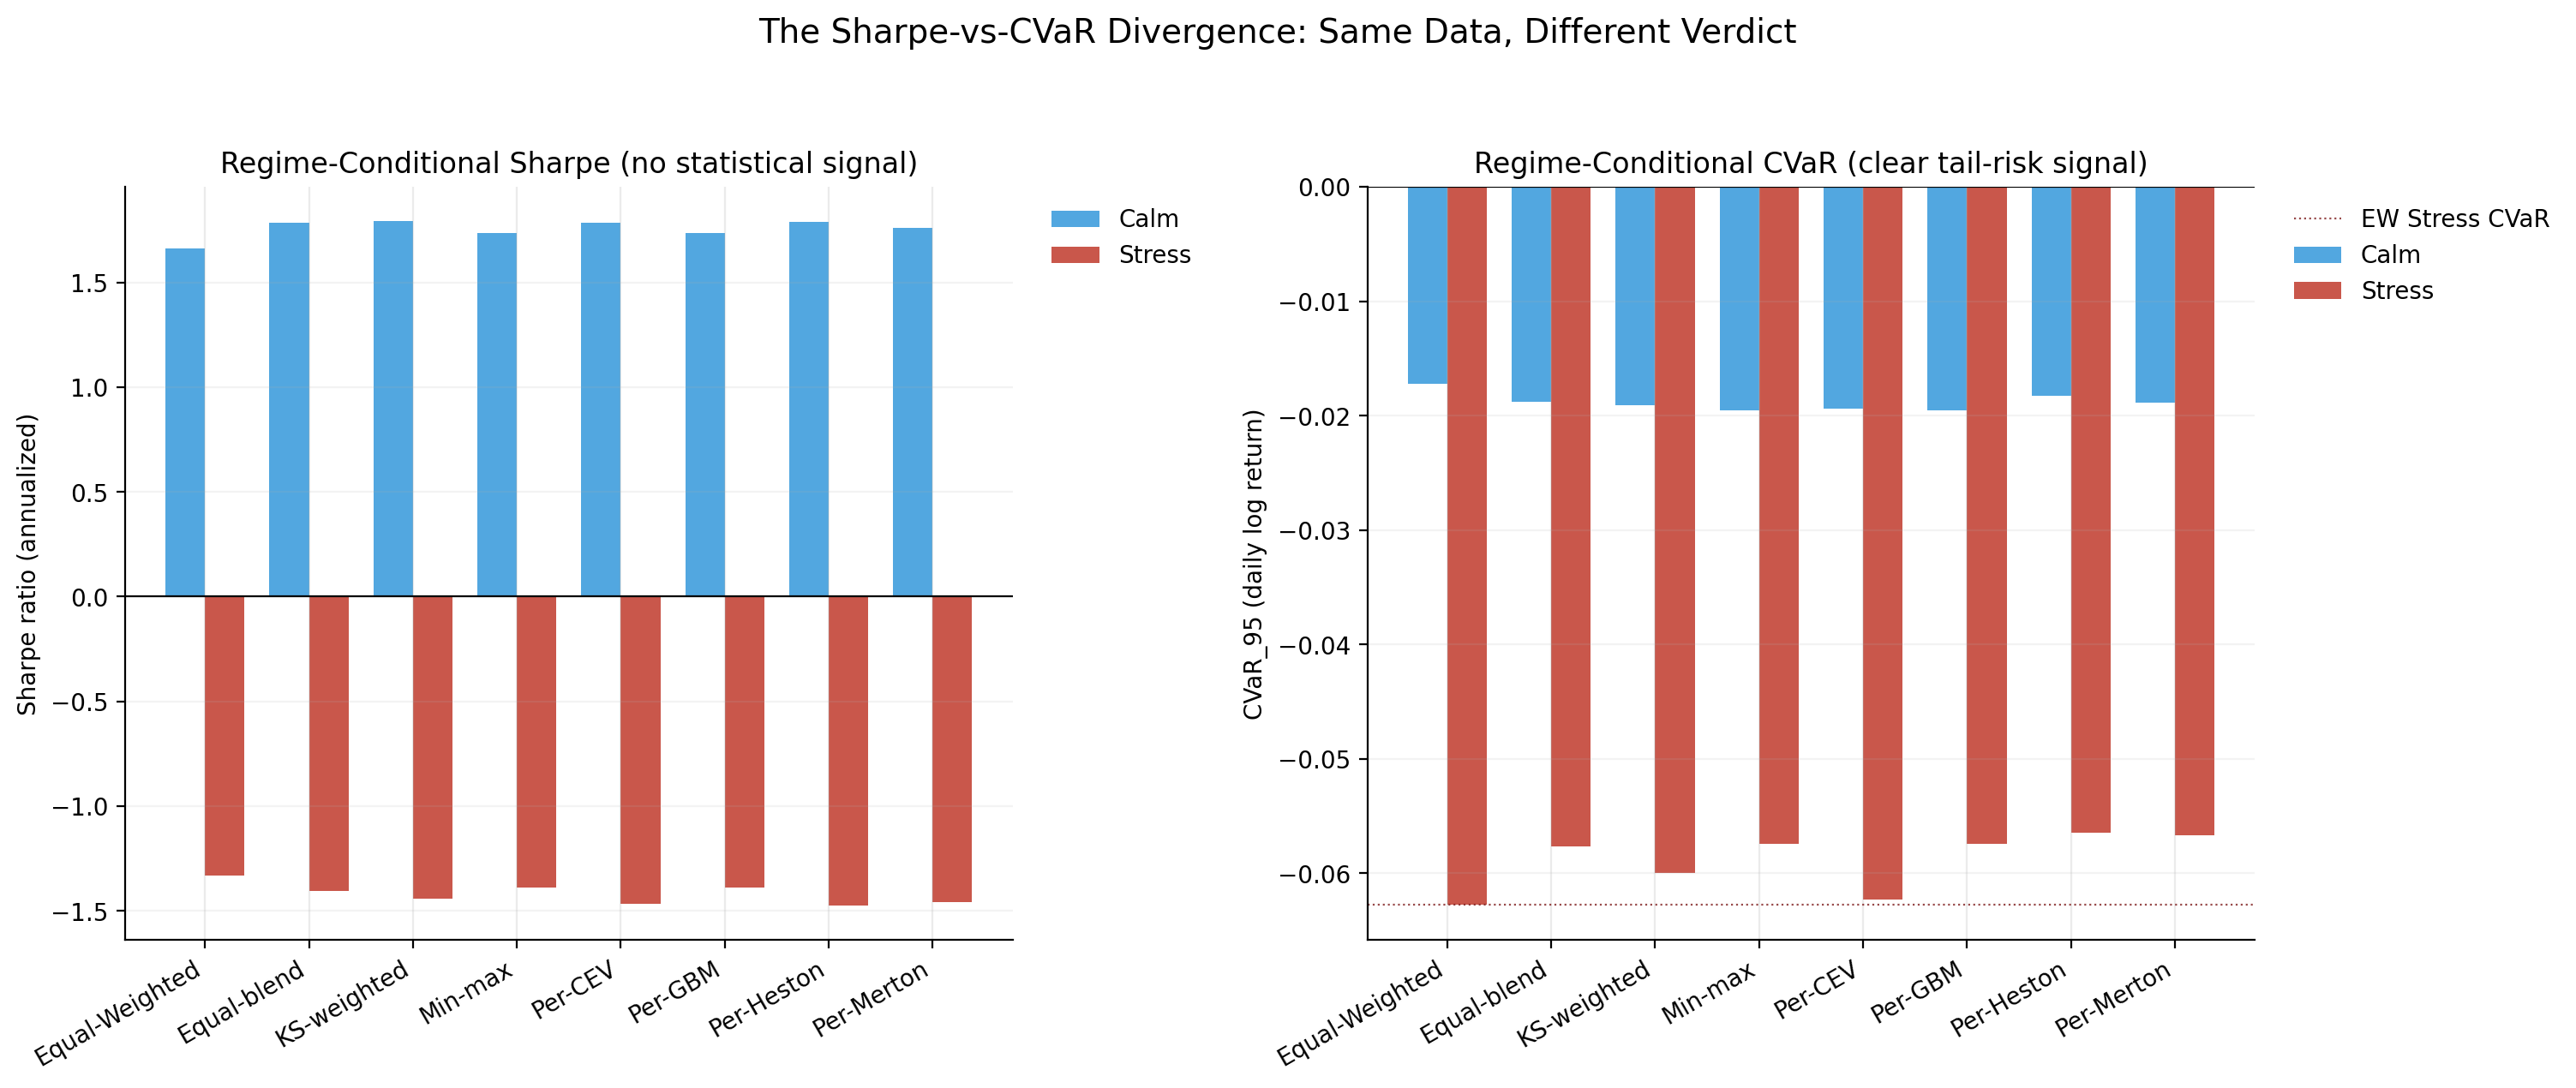
\includegraphics[width=0.95\textwidth]{figures/08_sharpe_vs_cvar_divergence.png}
\caption{The same data, evaluated through Sharpe ratio (left) versus through CVaR (right). The Sharpe panel shows no cross-portfolio signal; the CVaR panel shows a clear separation between the optimized portfolios and the Equal-Weighted benchmark in the Stress regime. The right panel's dotted line marks the EW Stress-CVaR reference. This is, in our view, the most important figure of this report.}
\label{fig:divergence}
\end{figure}

% =================================================================
% 9. Discussion
% =================================================================
\section{Discussion}

\subsection{Sharpe and CVaR Disagree, and the Disagreement Is Informative}

The cleanest reading of the joint Phase~6 / Phase~7 result is that Sharpe ratio and CVaR are measuring different things, and a strategy designed to manipulate one of them should be evaluated on that one. The Min-max worst-case formulation in Phase~4 maximizes the minimum Sharpe across model-conditional return distributions; this is a Sharpe-targeted objective at design time, but the hedge that the formulation effectively implements (by tilting toward GLD and capping equity concentration) operates on the left tail. Sharpe averages over both tails of the return distribution; CVaR conditions on the left tail. The fact that the Min-max portfolio shows no Sharpe advantage but does show a CVaR advantage in the regime where the left tail is most active is the expected signature of a left-tail-targeting overlay implemented (perhaps inadvertently) through model-uncertainty robustness.

This connects directly to the MGT 6081 framework on coherent risk measures \citep{artzner1999coherent, rockafellar2002conditional}. Sharpe ratio is not a coherent risk measure; it is not even a risk measure (it is a risk-adjusted return measure). CVaR is. For derivatives-overlay strategies and any other state-contingent payoff structure, the coherent measure is the appropriate evaluation metric, and conditioning on state (regime, in our framework) is intrinsic to the metric's interpretation.

\subsection{Which Models Are Pertinent for the Future?}

This subsection is our direct answer to the closing question of Project Idea~1: \emph{which models do you think are more pertinent for the future that is anticipated?}

In our opinion, the strongest model for forward-looking use within this universe is \textbf{Heston stochastic volatility}, with \textbf{Merton jump-diffusion} a close second. We base this on three pieces of evidence:

\textbf{Evidence 1: Stress-day CVaR performance.} The Per-Heston portfolio achieves the best Stress-day CVaR ($-5.65\%$) of all eight portfolios we evaluated, beating the Equal-Weighted benchmark by 62 bps per day. Per-Merton follows at 60 bps. These are the two largest improvements in the table. By contrast, Per-GBM and Min-max (which equals Per-GBM) achieve $+53$ bps; Per-CEV achieves only $+4$ bps. The relative ranking is Heston > Merton > GBM/Min-max > KS-weighted/Equal-blend > CEV. The two stochastic-volatility / jump-diffusion models meaningfully dominate the diffusion-only models on the metric that matters for tail-risk-aware portfolio construction.

\textbf{Evidence 2: Goodness-of-fit to empirical returns.} Heston and Merton track the empirical SPY return distribution's tails meaningfully better than GBM and CEV (Figure~\ref{fig:qq}). This matters because forward-looking portfolio construction should be anchored in models whose marginal distributions match the data. Heston captures stochastic volatility (vol-of-vol) and the leverage effect via $\rho < 0$; Merton explicitly models the discrete-event jumps that drive Stress regimes. GBM has neither; CEV's leverage effect is rigidly deterministic via $\beta$ and is empirically too weak.

\textbf{Evidence 3: Empirical relevance of stochastic volatility.} The HMM regime decomposition itself is direct empirical evidence that the SPY return process exhibits substantial volatility-of-volatility ($14.5\%$ Calm vs.\ $47.0\%$ Stress, switching with sticky transitions). A model that takes vol-of-vol seriously (Heston) is structurally aligned with this empirical fact in a way that GBM (constant $\sigma$) is not. The Heston parameters we calibrated have $\xi \approx 0.9$ for AAPL, indicating substantial uncertainty about future variance —which, again, is what the empirical regime structure independently confirms.

In our view, the right answer for forward-looking institutional use is not to pick a single model but to use the \emph{robust ensemble}. The Equal-blend, KS-weighted, and Min-max formulations all sit at or above the EW benchmark on Stress CVaR; the ensemble approach hedges against the (entirely realistic) possibility that we have specified the wrong single model. If a single-model view is required —which is what Project~1 asks for— our answer is Heston. If an ensemble view is permitted, we would deploy the Equal-blend for its conceptual simplicity and competitive Stress-CVaR performance ($+51$ bps).

\subsection{The DGU Puzzle Revisited}

\citet{demiguel2009optimal} found that a wide range of optimization techniques fail to beat $1/N$ on out-of-sample Sharpe. Phase~6 of this project reproduces that finding cleanly. Phase~7 does not refute it but reframes it: the optimization techniques may be doing what they were designed to do (manage tail risk in adverse regimes), and the failure is in the choice of evaluation metric, not in the optimization itself. This suggests an interpretation of the DGU puzzle as partly metric-mismatch: $1/N$ is hard to beat on Sharpe because Sharpe is the wrong metric for many of the alternatives being compared to it. We do not claim this fully resolves the DGU puzzle; we do claim that any future replication of the DGU experiment should report regime-conditional CVaR alongside unconditional Sharpe.

\subsection{Limitations and Honest Caveats}

We disclose the following limitations explicitly.

\textbf{In-sample inference for Phase~7.} The Phase~7 paired bootstrap is conducted on the training period, not on out-of-sample data. The honest reason is sample size: the 332-day OOS window contains only 15 HMM-identified Stress days, which is far below the minimum sample size required for stable bootstrap inference on Sharpe ratios. (For comparison, our training Stress sample is 145 days.) The Phase~7 OOS analysis is presented as descriptive only.

\textbf{Min-max degeneracy.} The Min-max optimizer converged to the same weight vector as the per-GBM portfolio, indicating that GBM was the binding worst-case model. This is an honest limitation of the formulation. The cross-portfolio L1 distance between Min-max and Per-GBM is exactly $0.000$. A truly informative min-max should select weights different from any per-model maximum-Sharpe portfolio. Possible causes we considered: (i) the $30\%$ per-asset cap interacts with GBM's particular risk-return geometry, making GBM the binding constraint; (ii) the four model-conditional Sharpes are too close together for the min-max to find an interior solution that improves on the worst case. Future work could investigate widening the ambiguity set, removing the cap, or adding a regularization term that penalizes corner solutions in the min-max objective.

\textbf{Bootstrap on regime-filtered series.} The block bootstrap on regime-conditional returns implicitly treats within-regime dynamics as homogeneous across spells, ignoring the discontinuities at regime boundaries. This is the standard approach in the regime-conditional inference literature and is unlikely to materially affect results, but it is worth noting.

\textbf{HMM specification.} A two-state HMM is a deliberate simplification. Three or four states could capture, e.g., a ``Crisis'' state distinct from a ``Stress'' state, at the cost of identification difficulty and reduced per-state sample size. We chose two states as the most parsimonious specification that produces externally validated regime labels.

\textbf{Asset universe.} Seven assets is a tractable problem size for a course project but is not representative of institutional portfolio construction, which would typically span hundreds of assets. The qualitative conclusions are likely robust to universe expansion; the specific quantitative results would change.

\textbf{No transaction costs or market impact.} Our portfolio NAV reconstruction assumes daily fixed-weight rebalancing at zero cost. In practice, a portfolio with the concentrated AAPL/GLD exposure of our optimized portfolios would incur material rebalancing costs at institutional scale. We did not model these.

\textbf{Single OOS window.} Our OOS evaluation uses a single 16-month window. A more rigorous evaluation would use a rolling-window or expanding-window cross-validation scheme, retraining the models periodically and aggregating across multiple OOS sub-windows. We did not do this because the training window was too short to support multiple disjoint sub-windows of meaningful size, and we believed it was more honest to report the single-window result transparently than to manufacture statistical power through window engineering.

% =================================================================
% 10. Conclusion
% =================================================================
\section{Conclusion}

This project implements and validates a multi-model robust portfolio optimization framework for a seven-asset universe, integrating the full set of components prescribed by Project Idea~1 (Markowitz baseline, four stochastic-process models, multi-model portfolio reoptimization, BSM options overlay) and substantially extending the validation framework along the lines that we believed —and the instructor approved— were necessary to qualify the work as Project Idea~6.

The empirical conclusion is two-part. \emph{Unconditionally}, the model-robust Min-max portfolio is statistically indistinguishable from the naïve $1/N$ benchmark on out-of-sample Sharpe ratio over a single 16-month window —a textbook \citet{demiguel2009optimal} result, which we report honestly. \emph{Conditional on regime}, the Sharpe-ratio finding survives, but the regime-conditional CVaR comparison reveals that the model-robust portfolios deliver measurable tail-risk reduction during Stress regimes (53–62 basis points per day for Min-max, Per-Heston, and Per-Merton) at a measurable cost in Calm-regime tail risk —the expected design signature of a tail-risk-insurance strategy.

The methodological takeaway is that strategies designed to manage state-contingent risk must be evaluated using state-contingent risk metrics. For derivative-overlay strategies and robust portfolios alike, the coherent risk measure (CVaR) conditioned on regime is the right evaluation object; the unconditional Sharpe ratio is not.

In direct response to Project~1's closing question, we conclude that the Heston stochastic-volatility model is the most pertinent single model for forward-looking portfolio construction within this universe (best Stress-CVaR performance), with Merton jump-diffusion a close second. The robust ensemble formulations (Equal-blend, KS-weighted) are competitive and should be preferred when single-model commitment is not required, since they hedge against model-misspecification risk by construction.

We end with what we hope is the project's most useful outcome for our own development: an honest, falsifiable framework for portfolio evaluation, in which negative findings are reported as readily as positive ones, and in which the choice of evaluation metric is treated as part of the scientific question rather than as an afterthought.

% =================================================================
% References
% =================================================================
\bibliographystyle{apalike}
\bibliography{references}

% =================================================================
% Appendices
% =================================================================
\appendix

\section{Project Repository Structure}

The complete project is publicly available at \url{https://github.com/anay-a-joshi/StochastiQ} under the MIT License. The directory layout is as follows.

\begin{lstlisting}[basicstyle=\small\ttfamily,frame=none]
StochastiQ/
|-- src/                              # production source code
|   |-- config.py                     # global constants (rf, trading days, seed)
|   |-- data/loaders.py               # yfinance ingestion, return computation
|   |-- models/                       # stochastic process implementations
|   |   |-- gbm.py
|   |   |-- merton.py
|   |   |-- cev.py
|   |   `-- heston.py
|   |-- simulation/monte_carlo.py     # Cholesky-correlated path generation
|   |-- optimization/
|   |   |-- markowitz.py              # Phase 2 mean-variance frontier
|   |   `-- robust.py                 # Phase 4 per-model + min-max + blends
|   |-- options/                      # Phase 5 BSM overlay
|   |   |-- bsm.py                    # Black-Scholes-Merton pricing
|   |   `-- strategies.py             # covered call, protective put, collar
|   |-- validation/bootstrap.py       # Politis-Romano stationary bootstrap
|   `-- regime/                       # Phase 7 HMM module
|       |-- detection.py              # 2-state Gaussian HMM with relabeling
|       `-- evaluation.py             # regime-conditional metrics
|-- notebooks/
|   |-- 01_data_pull.ipynb            # data ingestion, sanity checks
|   |-- 02_markowitz.ipynb            # mean-variance baseline
|   |-- 03_model_calibration.ipynb    # GBM/Merton/CEV/Heston fits
|   |-- 04_monte_carlo_robust_portfolios.ipynb
|   |-- 05_options_overlay.ipynb      # BSM strategies
|   |-- 06_out_of_sample_validation.ipynb  # bootstrap inference
|   |-- 07_regime_analysis.ipynb      # HMM + regime-conditional analysis
|   `-- 08_final_results.ipynb        # cross-phase aggregation
|-- data/processed/                   # parquet files (gitignored)
|-- reports/
|   |-- figures/                      # all generated PNGs (~30 figures)
|   |-- StochastiQ_Final_Report.tex   # this document
|   |-- references.bib                # bibliography
|   `-- build_report.sh               # one-command compile script
|-- requirements.txt                  # Python dependencies
|-- LICENSE                           # MIT
`-- README.md
\end{lstlisting}

The Git history is preserved with phase-by-phase commits, each pushing a self-contained, runnable contribution. The most recent commits, in chronological order, are: \texttt{5dbac85} (Phase~4), \texttt{c3127a8} (Phase~5), \texttt{a42d140} (Phase~6), \texttt{664d3df} (Phase~3 source patch), \texttt{21b7e4f} (Phase~7), and the Phase~8 commit (this report).

\section{Reproducibility}

All randomness is seeded with \texttt{RANDOM\_SEED = 42} from the project-level configuration in \texttt{src/config.py}. Specifically: the HMM is fit with \texttt{random\_state=42}, EM tolerance $10^{-6}$, maximum 1{,}000 iterations. Monte Carlo simulation uses 5{,}000 paths per model with \texttt{numpy.random.default\_rng(42)}. Block-bootstrap inference uses \texttt{seed=42}, $B = 5{,}000$ replicates, block length $\approx n^{1/3}$.

To reproduce all results from a clean clone of the repository:
\begin{lstlisting}[basicstyle=\small\ttfamily]
git clone https://github.com/anay-a-joshi/StochastiQ.git
cd StochastiQ
python -m venv venv && source venv/bin/activate
pip install -r requirements.txt
jupyter lab
# Run notebooks 01 through 08 in order.
\end{lstlisting}

Total runtime on a 2024-vintage Apple Silicon MacBook Pro is approximately 8 minutes for the full pipeline, dominated by the 5{,}000-replicate bootstrap in notebooks 06 and 07.

\section{Team Contribution Statement}

All four team members contributed substantively to the project. Specifically:

\begin{itemize}[leftmargin=*]
\item \textbf{Anay Abhijit Joshi} led the overall project architecture, the production source code under \texttt{src/}, the validation framework (Phase~6) and regime-conditional analysis (Phase~7), and the writing of this report.
\item \textbf{Vidhi Chaturvedi} led the Markowitz baseline (Phase~2), the cross-asset correlation analysis, and the goodness-of-fit evaluation (Phase~3 Q-Q plots).
\item \textbf{Sriya Nelluri} led the stochastic-process calibration (Phase~3), with primary responsibility for the Merton and Heston implementations, and contributed to the multi-model portfolio optimization (Phase~4).
\item \textbf{Himanshu Bhatt} led the BSM options overlay (Phase~5) including all three strategies, the Greek profiles, and the Sharpe-grid evaluation, and contributed to the discussion of options-overlay implications in Section~9.
\end{itemize}

All authors reviewed and approved the final report.

\end{document}
